\documentclass[10pt,aspectratio=1610,compress,dvipsnames]{beamer}
% --- Global figure numbering fix ---
\usepackage{etoolbox}
\usepackage{caption}
\usepackage{tikz}
\usepackage{comment}
%\usepackage{multimedia}
\usepackage{hyperref}
\usepackage{subcaption}
\usepackage{verbatim}
\captionsetup{font=footnotesize}
% Stop Beamer from resetting counters per frame

%new trial with new video
\usepackage{movie15}


\makeatletter
\let\beamer@reseteecounters=\relax
\pretocmd{\beamer@reseteecountersinframe}{\relax}{}{}
\makeatother

% Patch caption numbering (again, force global numbering)
\setbeamertemplate{caption}[numbered]
\addtocounter{figure}{0} % ensure figure counter is used globally

\usetheme[
%%% option passed to the outer theme
%    progressstyle=fixedCircCnt,   % fixedCircCnt, movingCircCnt (moving is deault)
  ]{Feather}

% Store the original frame environment
 
% If you want to change the colors of the various elements in the theme, edit and uncomment the following lines

% Change the bar colors:
%\setbeamercolor{Feather}{fg=red!20,bg=red}

% Change the color of the structural elements:
%\setbeamercolor{structure}{fg=red}

% Change the frame title text color:
%\setbeamercolor{frametitle}{fg=blue}

% Change the normal text color background:
%\setbeamercolor{normal text}{fg=black,bg=gray!10}

%-------------------------------------------------------
% INCLUDE PACKAGES
%-------------------------------------------------------

\usepackage[utf8]{inputenc}
\usepackage[spanish,es-tabla]{babel}
\usepackage[T1]{fontenc}
\usepackage{helvet}
%-------------------------------------------------------
% DEFFINING AND REDEFINING COMMANDS
%-------------------------------------------------------

% colored hyperlinks
\newcommand{\chref}[2]{
  \href{#1}{{\usebeamercolor[bg]{Feather}#2}}
}

\makeatletter
\def\blfootnote{\gdef\@thefnmark{}\@footnotetext}
\makeatother

%-------------------------------------------------------
% INFORMATION IN THE TITLE PAGE
%-------------------------------------------------------

\title[] % [] is optional - is placed on the bottom of the sidebar on every slide
{ % is placed on the title page
      \textbf{Optical tweezers implementation for a single-cell study of Diatoms:}
}

\subtitle[]
{
      \textbf{\small Exploration of trapping performance and the photonic properties of frustules}
}

\author[FC]
{      \textbf{\large Autor: Raymundo Vazquez Martinez} \\ \vspace{0.2cm}
      {\ttfamily Asesor: Dr. Remigio Cabrera Trujillo}
}

\institute[UNAM]
{
      \textbf{Universidad Nacional Autónoma de México}\\
      %Departamento de Física y Química Teórica\\
      Facultad de Ciencias\\
      %\vspace{0.2cm}
      %\includegraphics[scale=0.15]{logo}
      \vspace{-1cm}
  
  %there must be an empty line above this line - otherwise some unwanted space is added between the university and the country (I do not know why;( )
}

\date{\today}

%-------------------------------------------------------
% THE BODY OF THE PRESENTATION
%-------------------------------------------------------

\begin{document}

%-------------------------------------------------------
% THE TITLEPAGE
%-------------------------------------------------------

{\1% % this is the name of the PDF file for the background
\begin{frame}[plain,noframenumbering] % the plain option removes the header from the title page, noframenumbering removes the numbering of this frame only
  \titlepage % call the title page information from above
\end{frame}}


%-------------------------------------------------------
\section{Introducción}
%-------------------------------------------------------
% ----------------- Frame 1 -----------------
\begin{frame}<1-3>
  \frametitle{Introducción}
  \framesubtitle{La presión de radiación}

  \only<1>{
    La radiación electromagnética ejerce fuerza sobre los objetos materiales debido al intercambio de momento.
  }
\only<2>{

 \frametitle{Introducción}
  \framesubtitle{Resumen cronológico.}
  \only<1>{ 
  \begin{itemize}
    \item Siglo XVI: Idea de la presión de radiación de Kepler para explicar la orientación de los cometas.
    \item 1860s: Teoría electromagnética de Maxwell, primer sustento teórico para la presión de radiación.
    \item 1900s: Mediciones de la presión de radiación, por Albert Michelson y Francis Pease.
    \item 1960: Invención del láser por Theodore Maiman.
    \item 1970s: Primeros experimentos de Ashkin con partículas sintéticas.
    \item 1986: Invención de las pinzas ópticas por Arthur Ashkin y ejecucion luminica de bacterias.
    \item 2018: Premio Nobel de Física para Arthur Ashkin por su trabajo con las pinzas ópticas.
  \end{itemize}
  }
  \only<2>{
  \begin{itemize}
    \item Siglo XVI: Idea de la presión de radiación de Kepler para explicar la orientación de los cometas.
    \item 1860s: Teoría electromagnética de Maxwell, primer sustento teórico para la presión de radiación.
    \item 1900s: Mediciones de la presión de radiación, Albert Michelson y Francis Pease realizaron la primera medición directa.
    \item 1960: Invención del láser por Theodore Maiman.
    \ \fbox{\begin{minipage}{.9\textwidth} 
        \item 1970s: Primeros experimentos de Ashkin con partículas sintéticas. 
        \item 1986: Invención de las pinzas ópticas por Arthur Ashkin y ejecucion luminica de bacterias
      \end{minipage}}
    \item 2018: Premio Nobel de Física para Arthur Ashkin por su trabajo con las pinzas ópticas.
  \end{itemize}
  }

}
  \only<3>{
    La primera vez que se planteó que la presión de radiación podría explicar un fenómeno fue propuesta por Kepler.

    \refstepcounter{figure} % Incrementa figura globalmente
    \centering
    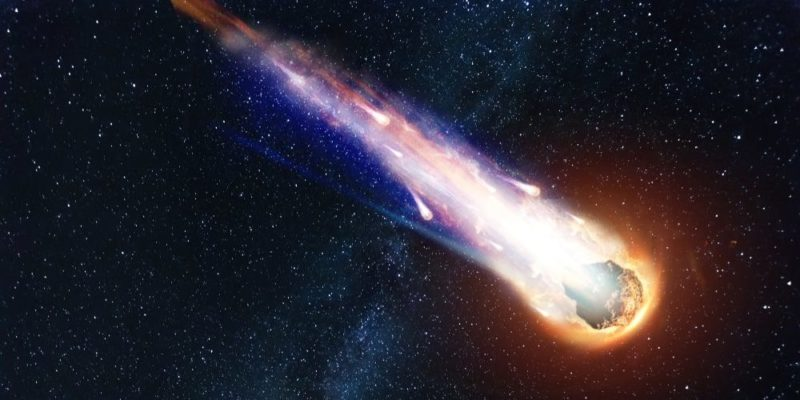
\includegraphics[width=0.5\linewidth]{cometa-e1561938278988.jpg}

    \vspace{0.5em}
    \textbf{Figura \arabic{figure}}:
    Un cometa que orbita alrededor del sol apunta su cola en dirección opuesta al mismo.
  }

 % \only<3>{
  %  El primer sustento teórico vino de la teoría electromagnética de Maxwell.
  %}

  %\only<4>{
   % Con las fuentes "naturales" de radiación, los fenómenos donde la presión de radiación jugaba un papel determinante eran astronómicos. 

    %\refstepcounter{figure}
    %\centering
    %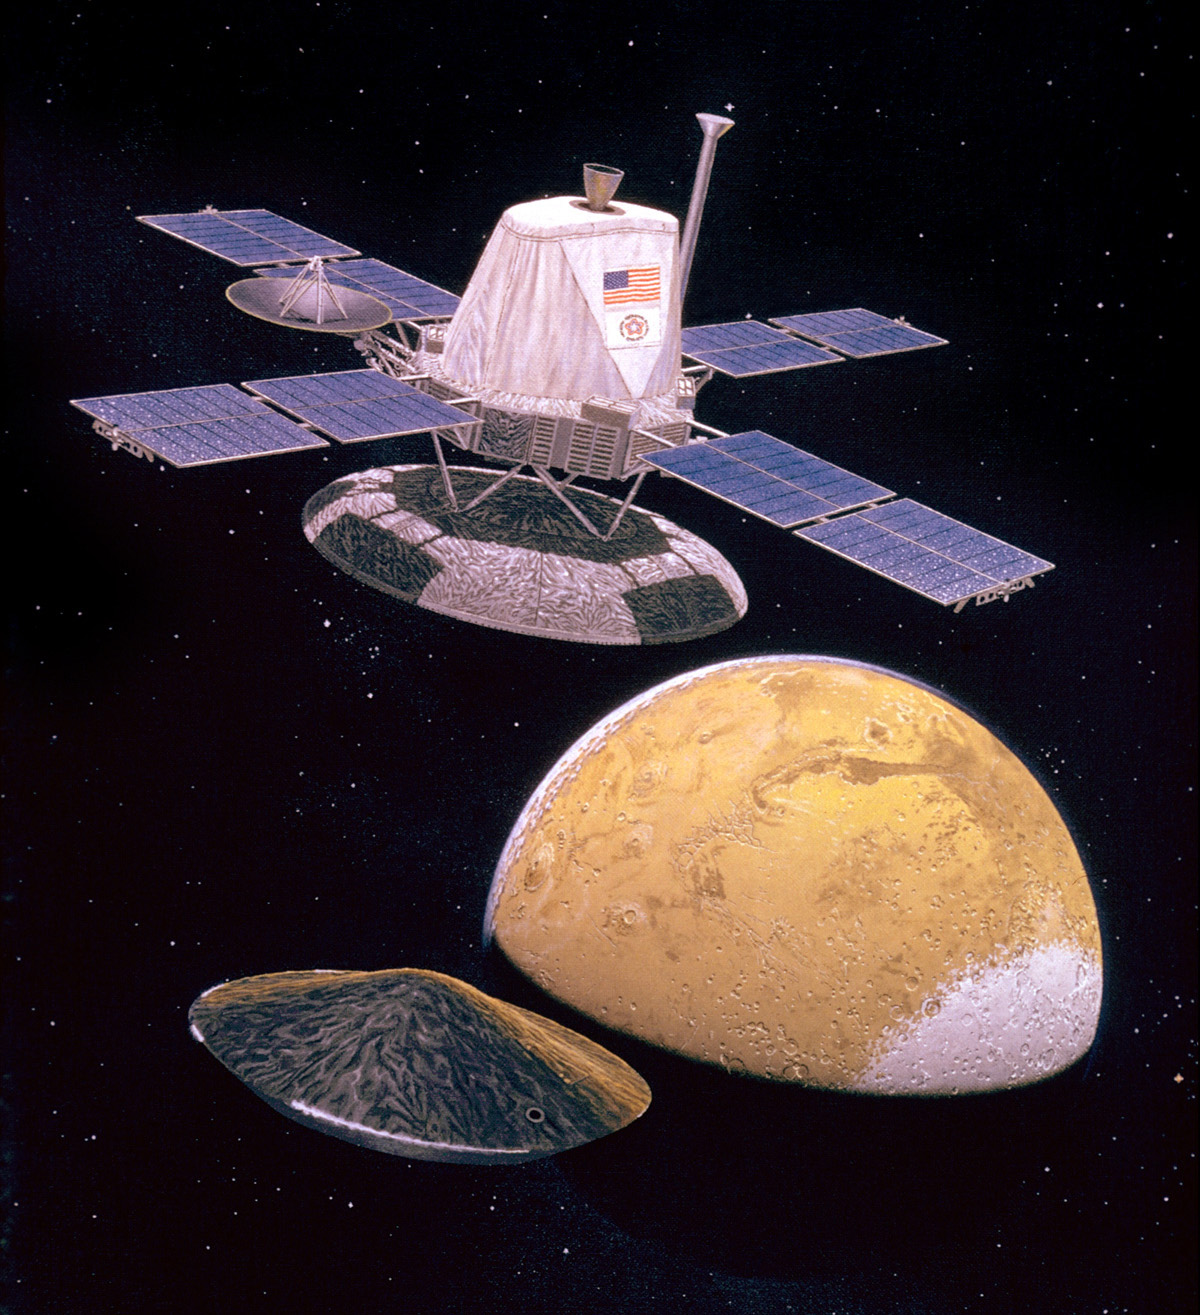
\includegraphics[scale=0.4]{Imagenes introduccion/Viking_Orbiter_releasing_the_lander.jpg}

    %\vspace{0.5em}
    %\textbf{Figura 2}: Un ejemplo de la modernidad:
    %La correcion de trayectoria de la mision viking.
  %}
  %\only<5>{
    
    %Con las fuentes "naturales" de radiación, los fenómenos donde la presión de radiación jugaba un papel determinante eran astronómicos. 

   % \refstepcounter{figure}
    %\centering
    %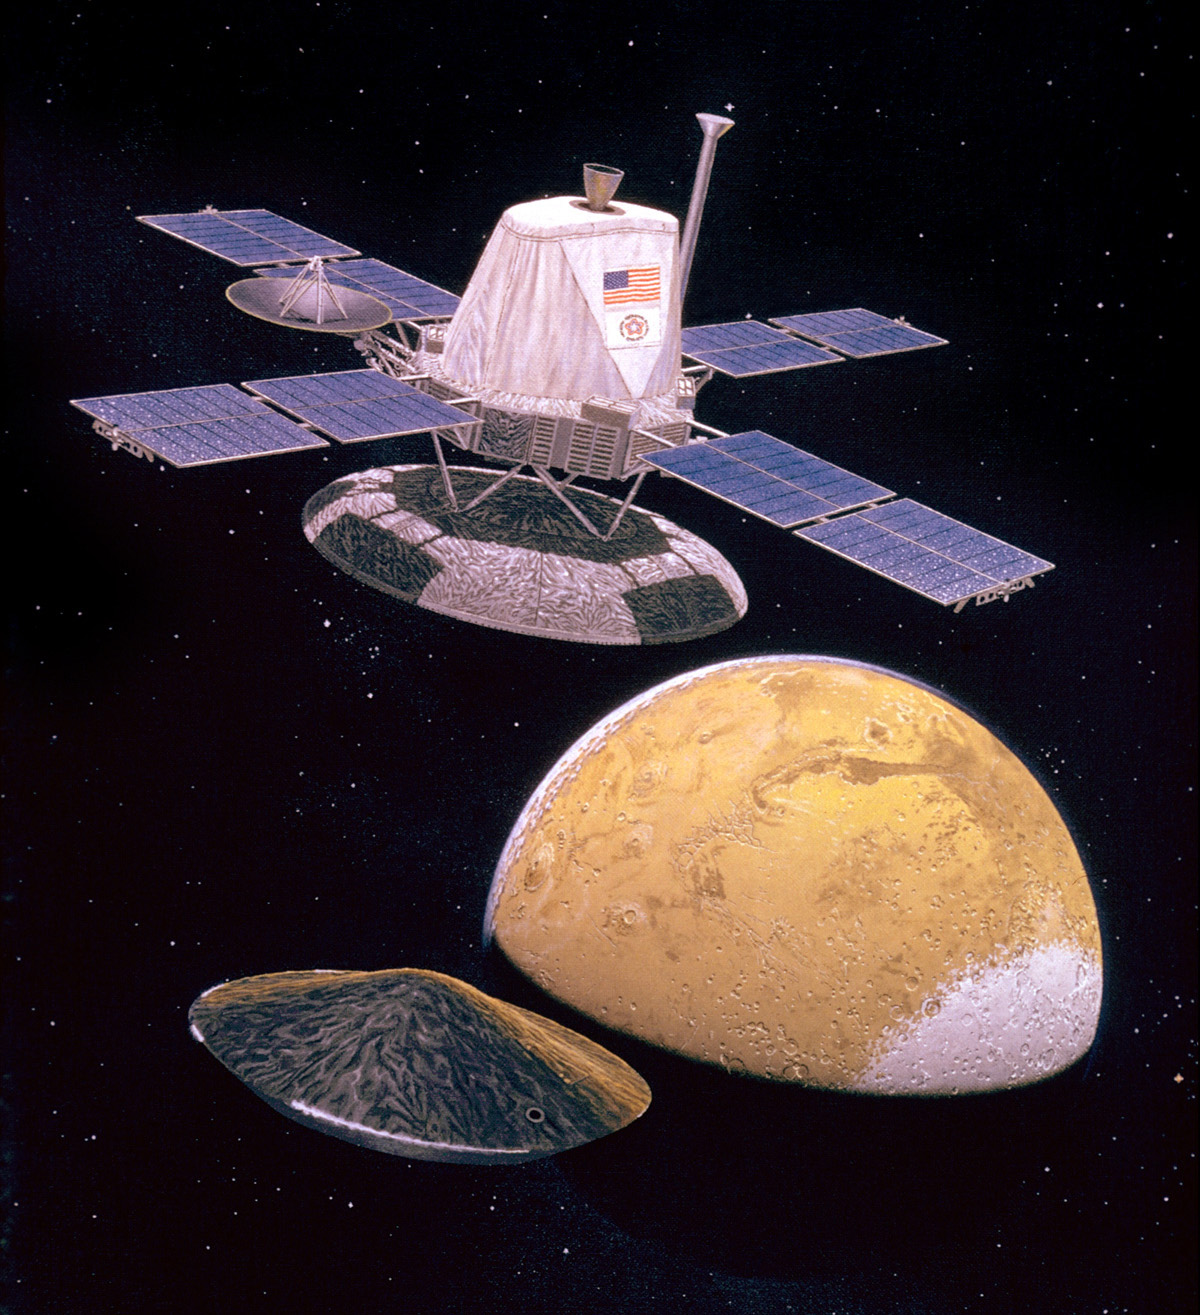
\includegraphics[scale=0.4]{Imagenes introduccion/Viking_Orbiter_releasing_the_lander.jpg}

    %\vspace{0.5em}
    %\textbf{Figura 2}: Un ejemplo de la modernidad:
    %La correcion de trayectoria de la mision viking.
  %}
%\end{frame}

%\begin{frame}<1-3>
 % \frametitle{Introducción}
  %\framesubtitle{El láser y las contribuciones de Ashkin.}

  %\only<1>{
   % La llegada del láser permitió, por primera vez, demostrar experimentalmente la aplicación de la \textbf{presión de radiación} en la manipulación de objetos en el laboratorio.
  %}

  %\only<2>{
   % Esto llevaría al desarrollo de las \textbf{pinzas ópticas}.
  %}
%\begin{comment} \only<3>{
    %Arthur Ashkin seria el pionero en estos desarrollos y recibiria el premio Nobel de Fisica en el 2018 
    
    %\refstepcounter{figure}
    %\centering
    %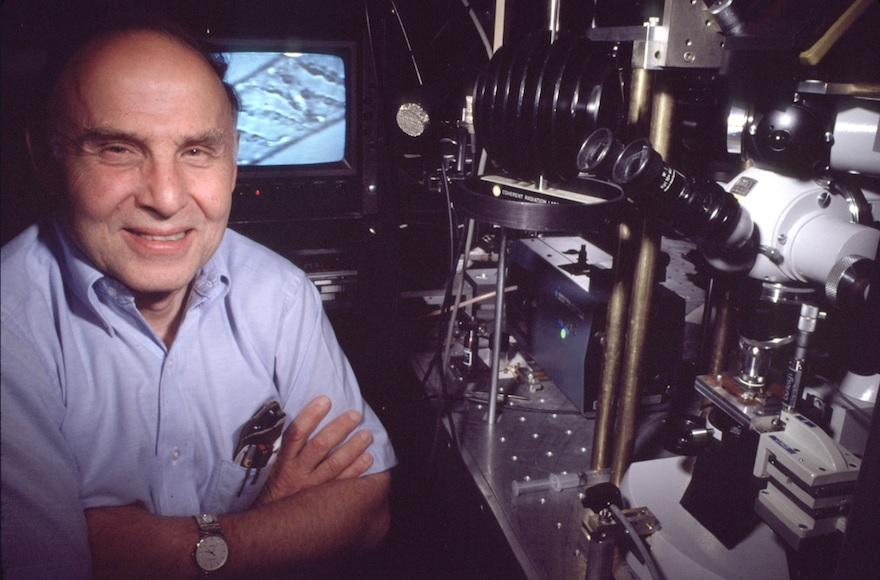
\includegraphics[scale=0.25]{Imagenes introduccion/NobelFis201801.jpg}

   % \vspace{0.5em}
  %  \textbf{Figura 2}: Arthur Ashkin en Bell labs..
 % }
  
  
\end{frame}


\begin{frame}<1-2>
  %-------------------------------------------------------
  \frametitle{Introducción}
  \framesubtitle{Resumen cronológico.}
  \only<1>{ 
  \begin{itemize}
    \item Siglo XVI: Idea de la presión de radiación de Kepler para explicar la orientación de los cometas.
    \item 1860s: Teoría electromagnética de Maxwell, primer sustento teórico para la presión de radiación.
    \item 1900s: Mediciones de la presión de radiación, por Albert Michelson y Francis Pease.
    \item 1960: Invención del láser por Theodore Maiman.
    \item 1970s: Primeros experimentos de Ashkin con partículas sintéticas.
    \item 1986: Invención de las pinzas ópticas por Arthur Ashkin y ejecucion luminica de bacterias.
    \item 2018: Premio Nobel de Física para Arthur Ashkin por su trabajo con las pinzas ópticas.
  \end{itemize}
  }
  \only<2>{
  \begin{itemize}
    \item Siglo XVI: Idea de la presión de radiación de Kepler para explicar la orientación de los cometas.
    \item 1860s: Teoría electromagnética de Maxwell, primer sustento teórico para la presión de radiación.
    \item 1900s: Mediciones de la presión de radiación, Albert Michelson y Francis Pease realizaron la primera medición directa.
    \item 1960: Invención del láser por Theodore Maiman.
    \ \fbox{\begin{minipage}{.9\textwidth} 
        \item 1970s: Primeros experimentos de Ashkin con partículas sintéticas. 
        \item 1986: Invención de las pinzas ópticas por Arthur Ashkin y ejecucion luminica de bacterias
      \end{minipage}}
    \item 2018: Premio Nobel de Física para Arthur Ashkin por su trabajo con las pinzas ópticas.
  \end{itemize}
  }
\end{frame}








 
%----------------------------------------
\section{Marco teórico}

\begin{frame}<1-8>
\frametitle{Marco teórico}
\framesubtitle{Diatomeas}
\only<1>{Las diatomeas son organismos unicelulares que se encuentran en la mayoria de los cuerpos de agua en la tierra.
}


\only<2>{
   \begin{figure}
      \centering
      \begin{subfigure}[b]{0.22\textwidth}
        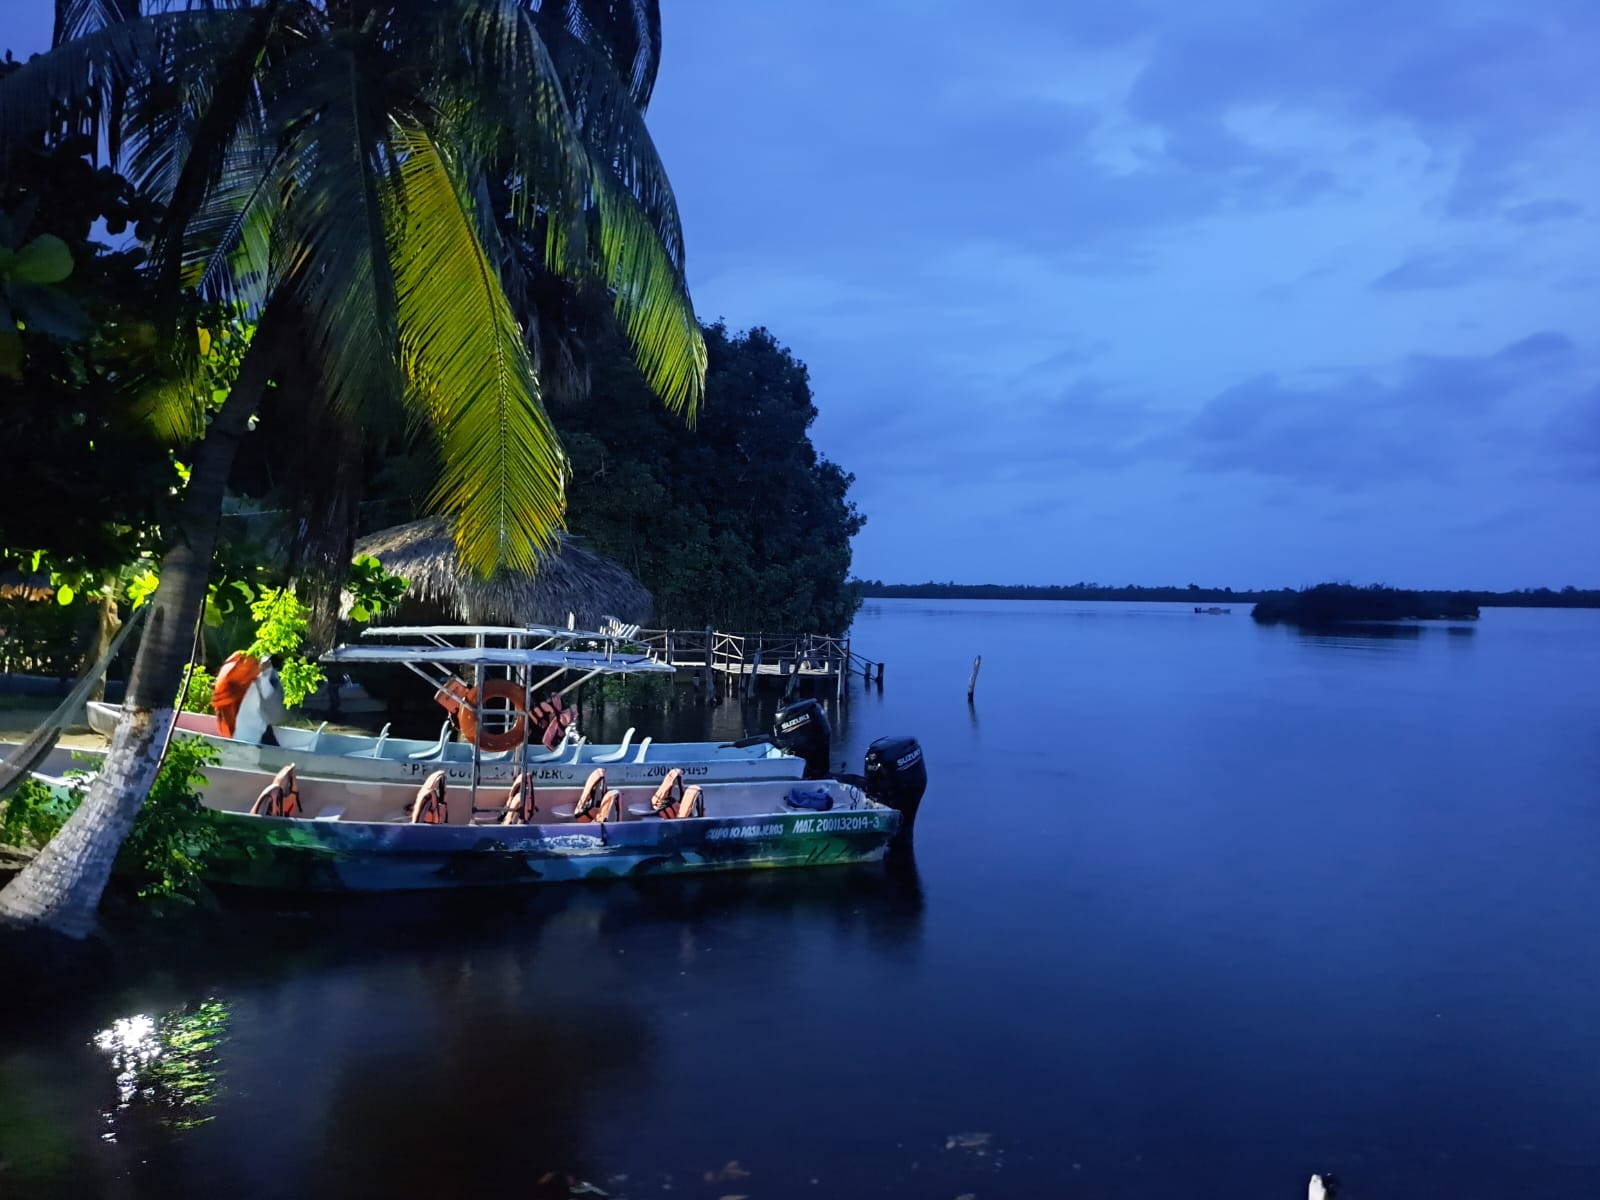
\includegraphics[width=\textwidth]{lago.jpeg}
        \caption*{\textbf{(a)}} % Pie de foto vacío, pero con la etiqueta
        \label{fig:sub1}
      \end{subfigure}\hspace{0.22cm}
      \begin{subfigure}[b]{0.22\textwidth}
        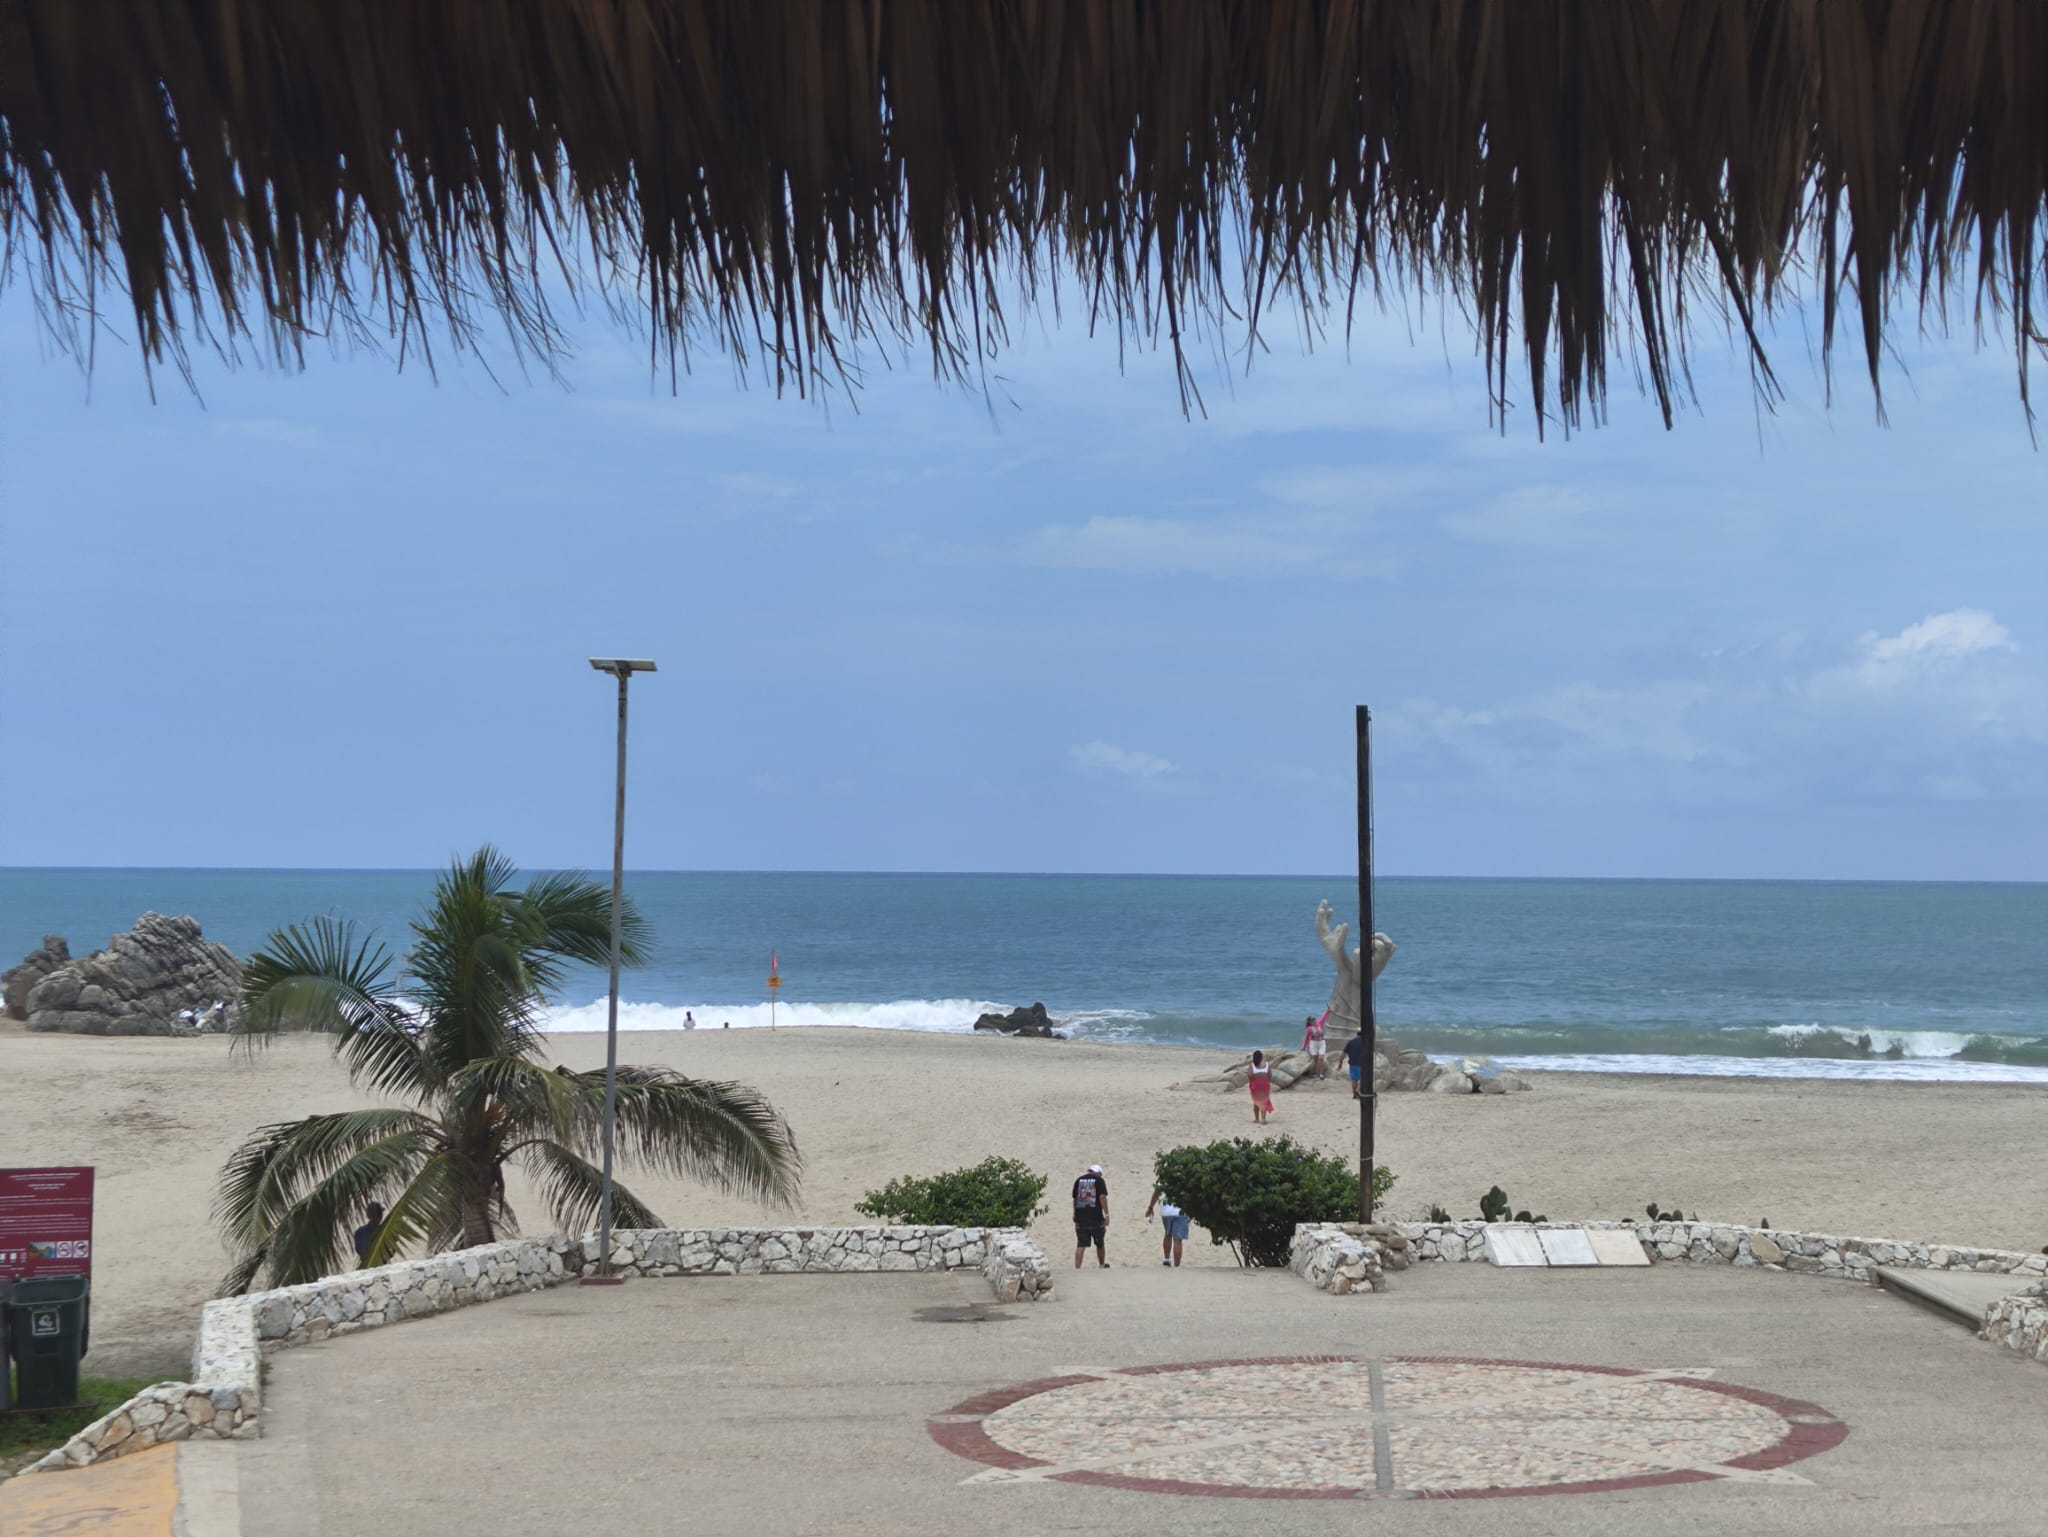
\includegraphics[width=\textwidth]{mar.jpeg}
        \caption*{\textbf{(b)}} % Pie de foto vacío, pero con la etiqueta
        \label{fig:sub2}
      \end{subfigure}

      \vspace{\baselineskip}

      \begin{subfigure}[b]{0.22\textwidth}
        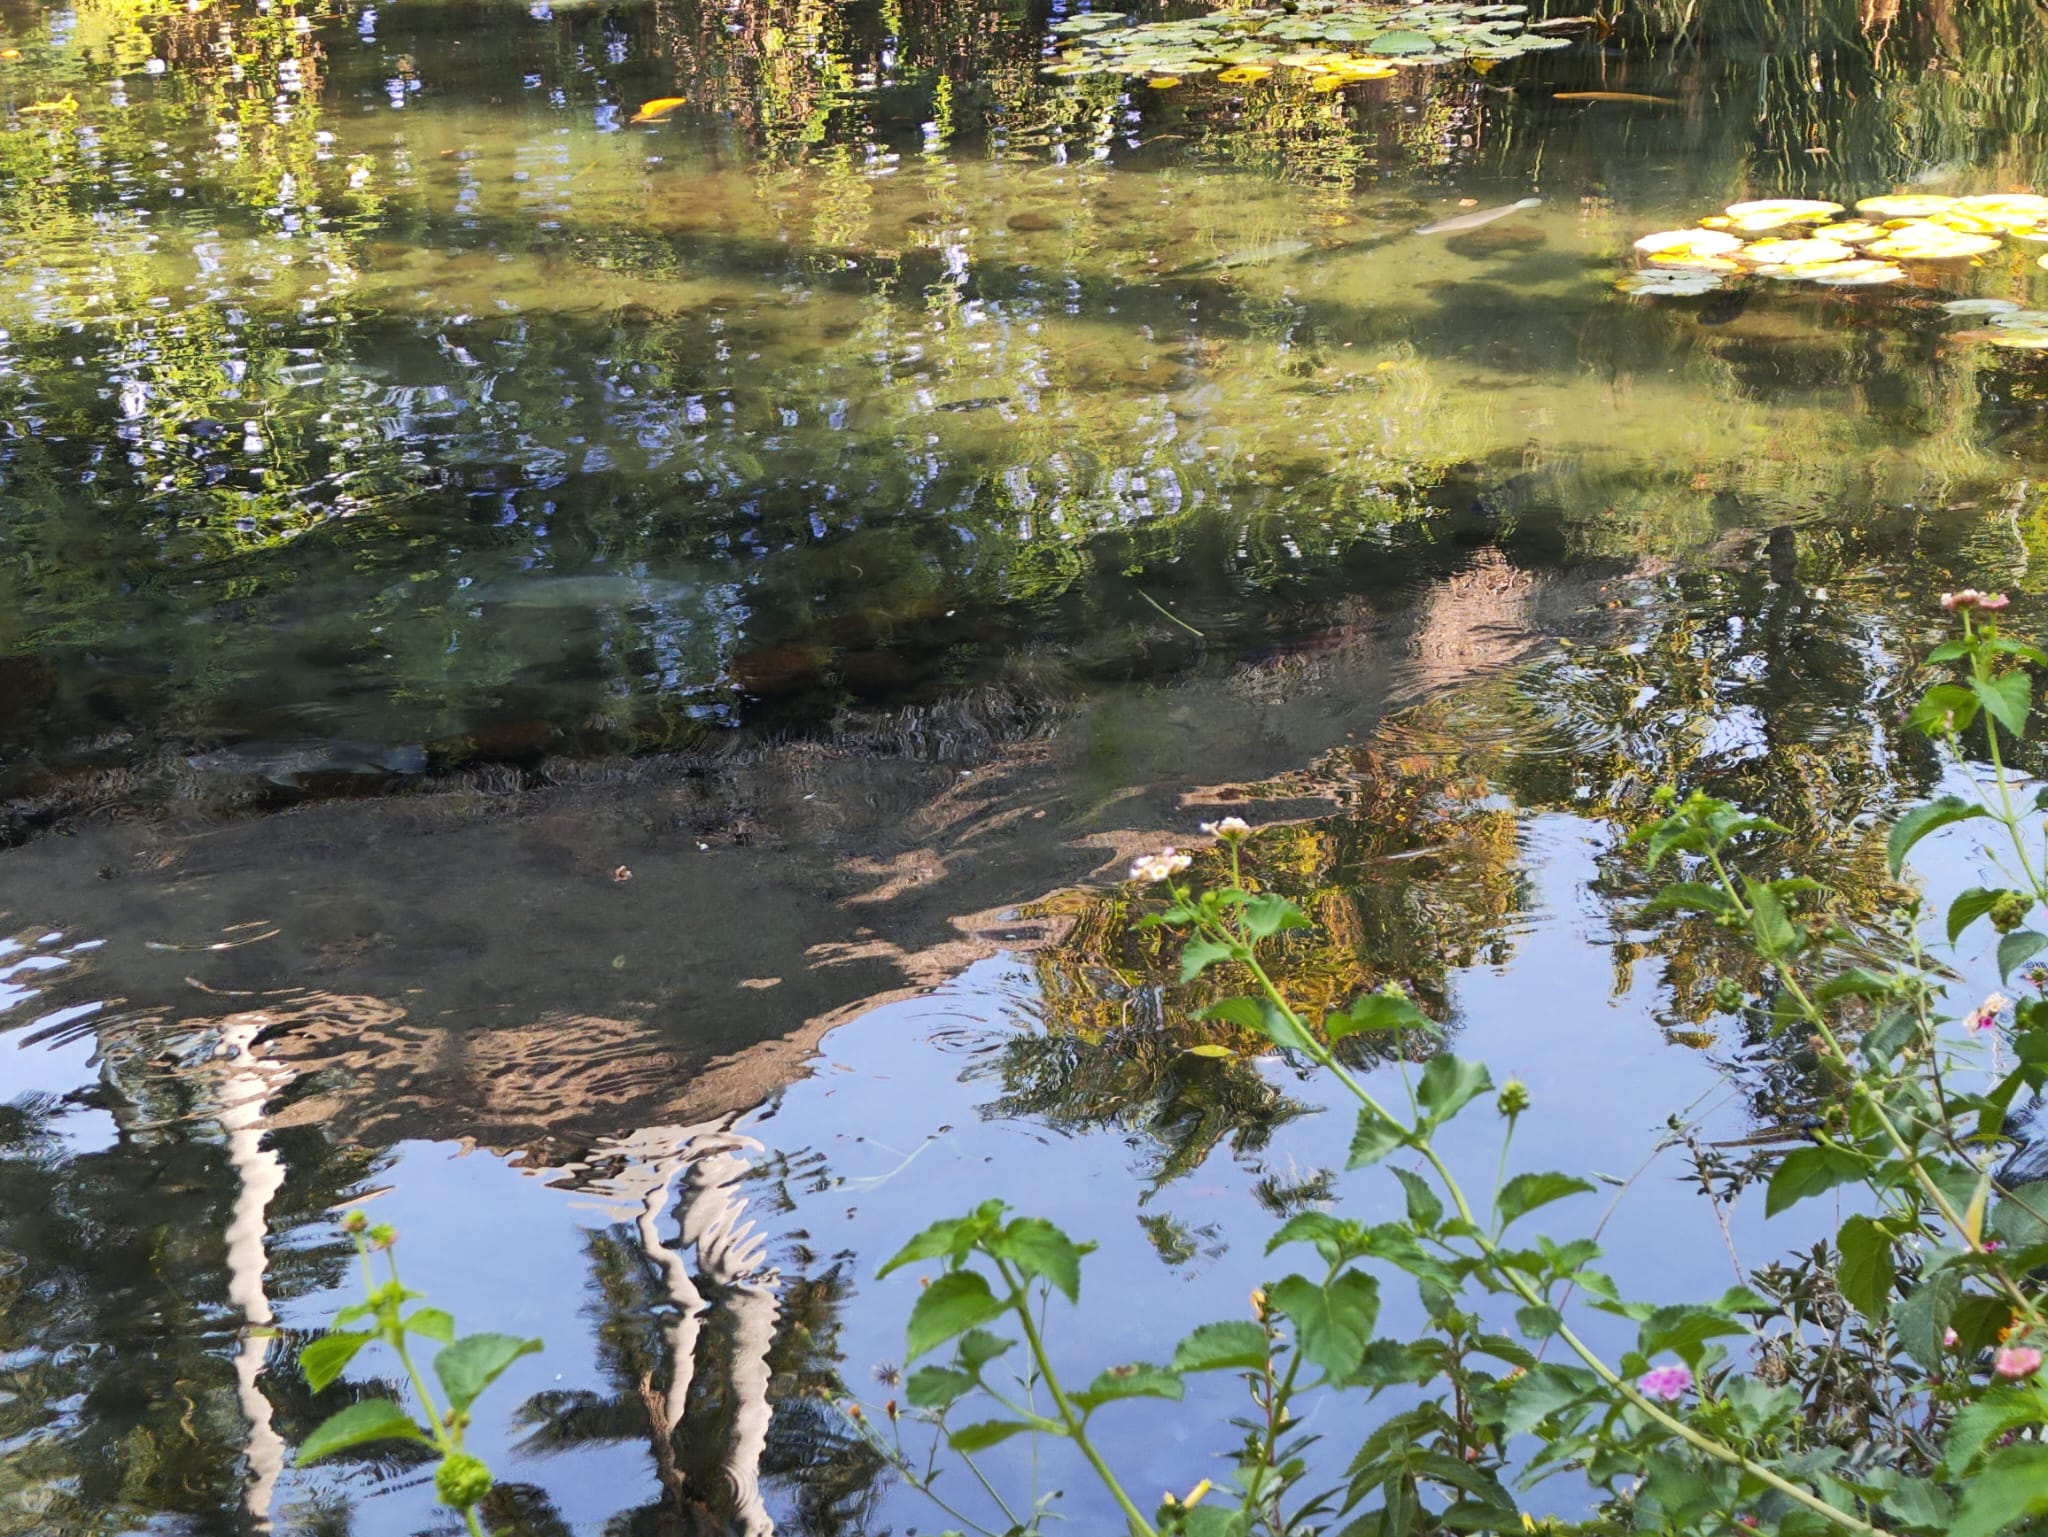
\includegraphics[width=\textwidth, height=2.2cm]{lodo.jpeg}
        \caption*{\textbf{(c)}} % Pie de foto vacío, pero con la etiqueta
        \label{fig:sub3}
      \end{subfigure}\hspace{0.5cm}
      \begin{subfigure}[b]{0.22\textwidth}
        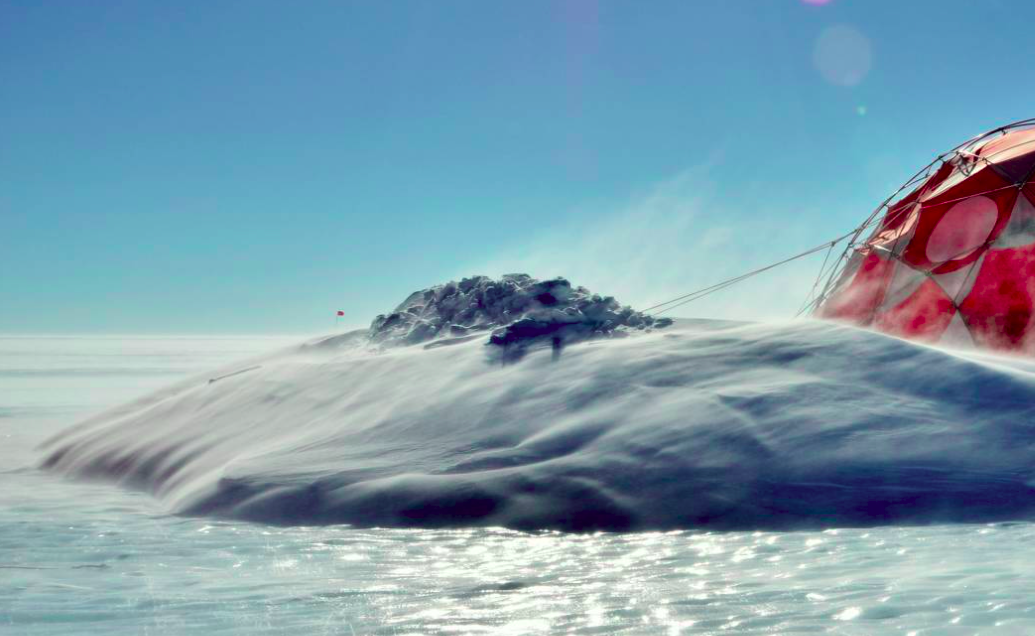
\includegraphics[width=\textwidth, height=2.2cm]{ice.png}
        \caption*{\textbf{(d)}} % Pie de foto vacío, pero con la etiqueta
        \label{fig:sub4}
      \end{subfigure}
      \caption{Se han encontrado diatomeas en \textbf{Lagos} (a) y \textbf{Mares} (b), en cuerpos de agua efimeras como \textbf{tierra humeda (c)} e incluso en \textbf{Nucleos de hielo en la antartica}}
      \label{fig:cuatro_subfiguras}
    \end{figure}
  }

\only<3>{Las diatomeas son organismos unicelulares que se encuentran en la mayoria de los cuerpos de agua en la tierra.
\vspace{0.7cm}
{Propiedades que hacen interesantes a las diatomeas: 

\begin{itemize}
    \item Organismos unicelulares fotosinteticos
    \item Grandes contribuidores de oxigeno ($20 - 25 \%$ del global)
    \item Gran variedad de especies: mas de 100 000 especies identificadas. 
    \item Valuadores historicos (debido a su acumulacion). 
    \item indicadores ambientales (debido a su variedad)
    \item Parte escencial de la cadena alimenticia acuatica.
    %\item Frustule synthesized from monosilicic acid
    %\item Frustule surface with micro- and nano-perforations (pores)
    %\item Frustule provides potential UV protection==
    %\item Frustule provides mechanical protection
    %\item High capacity for light harvesting
   % \item Significant oxygen producers (20-25\% globally)
    %\item Frustule exhibits photonic bandgap-like structures
    %\item Potential applications in solar cell enhancement
    %\item Over 100,000 identified species
    %\item Categorized by frustule symmetry (centric and pennate)
    %\item Accumulation leads to diatomaceous earth
    %\item Essential part of the aquatic food web
    %\item Frustule can modify coherent laser light
\end{itemize}}
}
\only<4>{\framesubtitle{Frustula} De suma importancia es notar la interaccion fructifera de las diatomeas con la luz.

{\vspace{0.8cm} Investigaciones se han hecho sobre la interaccion de la luz con las diatomeas. En las cuales la frustula ha sido de particular interes.}}
%Las propiedades de las diatomeas no solo se limitan a la ecologia.\newline


\only<5>{
Las frustulas son un caparazon de silica que aparece en la etapa de crecimiento de la alga y establece una  clasificacion binaria dada por la simetria de las frustulas.
   
   \vspace{1cm}
   \

}

\only<6>{

   \begin{figure}
      \centering
      \begin{subfigure}[b]{0.3\textwidth}
        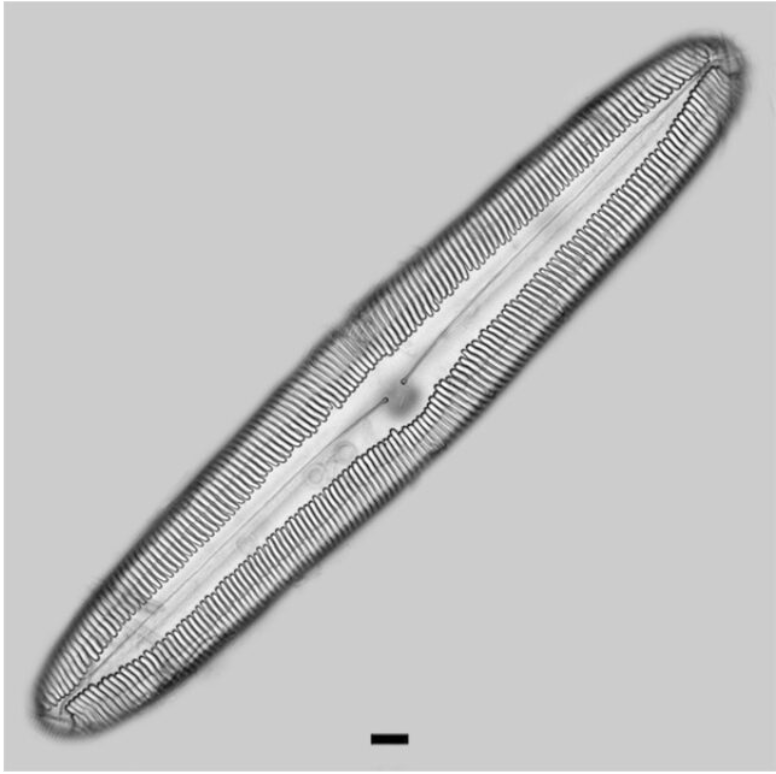
\includegraphics[width=\textwidth, height=2.2cm]{pen1.png}
        \caption*{\textbf{(a) \textit{Pinnularia dariana} }} % Pie de foto vacío, pero con la etiqueta
        \label{fig:sub1}
      \end{subfigure}\hspace{0.5cm}
      \begin{subfigure}[b]{0.3\textwidth}
        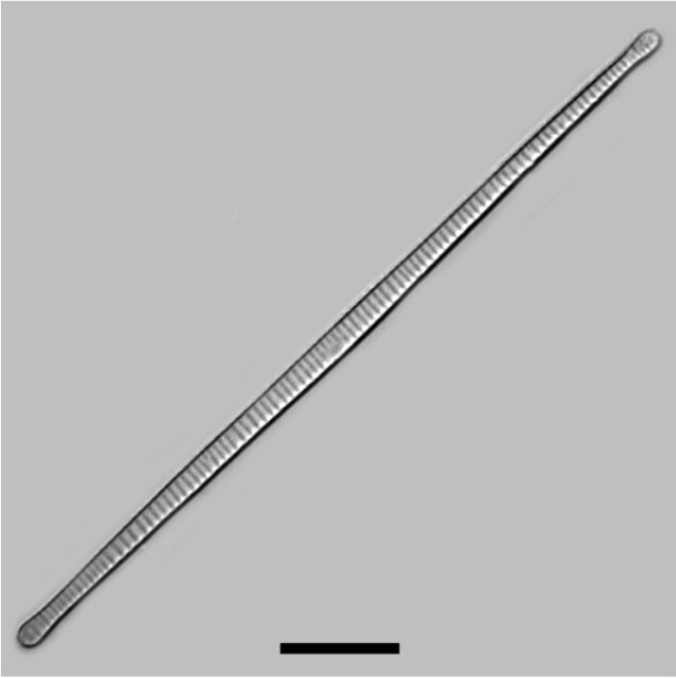
\includegraphics[width=\textwidth, height=2.2cm]{pen2.png}
        \caption*{\textbf{(b) \textit{Fragilaria synegrotesca}}} % Pie de foto vacío, pero con la etiqueta
        \label{fig:sub2}
      \end{subfigure}

      \vspace{\baselineskip}

      \begin{subfigure}[b]{0.3\textwidth}
        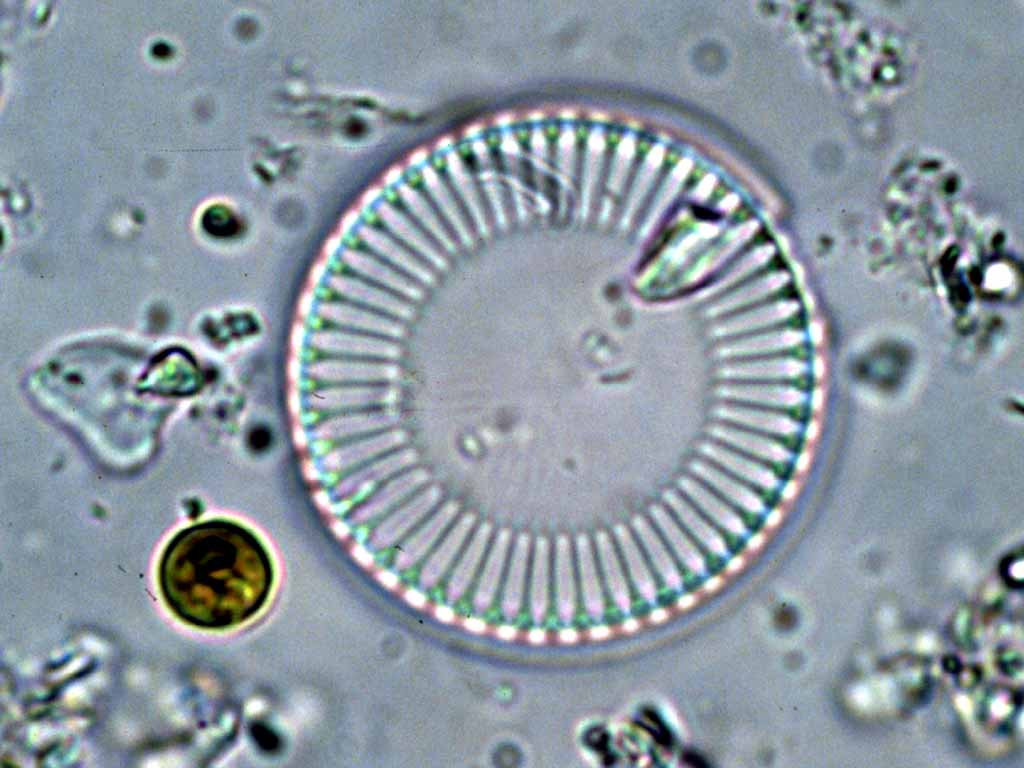
\includegraphics[width=\textwidth, height=2.2cm]{cen1.jpeg}
        \caption*{\textbf{(c) \textit{Cyclotella meneghiniana}}} % Pie de foto vacío, pero con la etiqueta
        \label{fig:sub3}
      \end{subfigure}\hspace{0.5cm}
      \begin{subfigure}[b]{0.3\textwidth}
        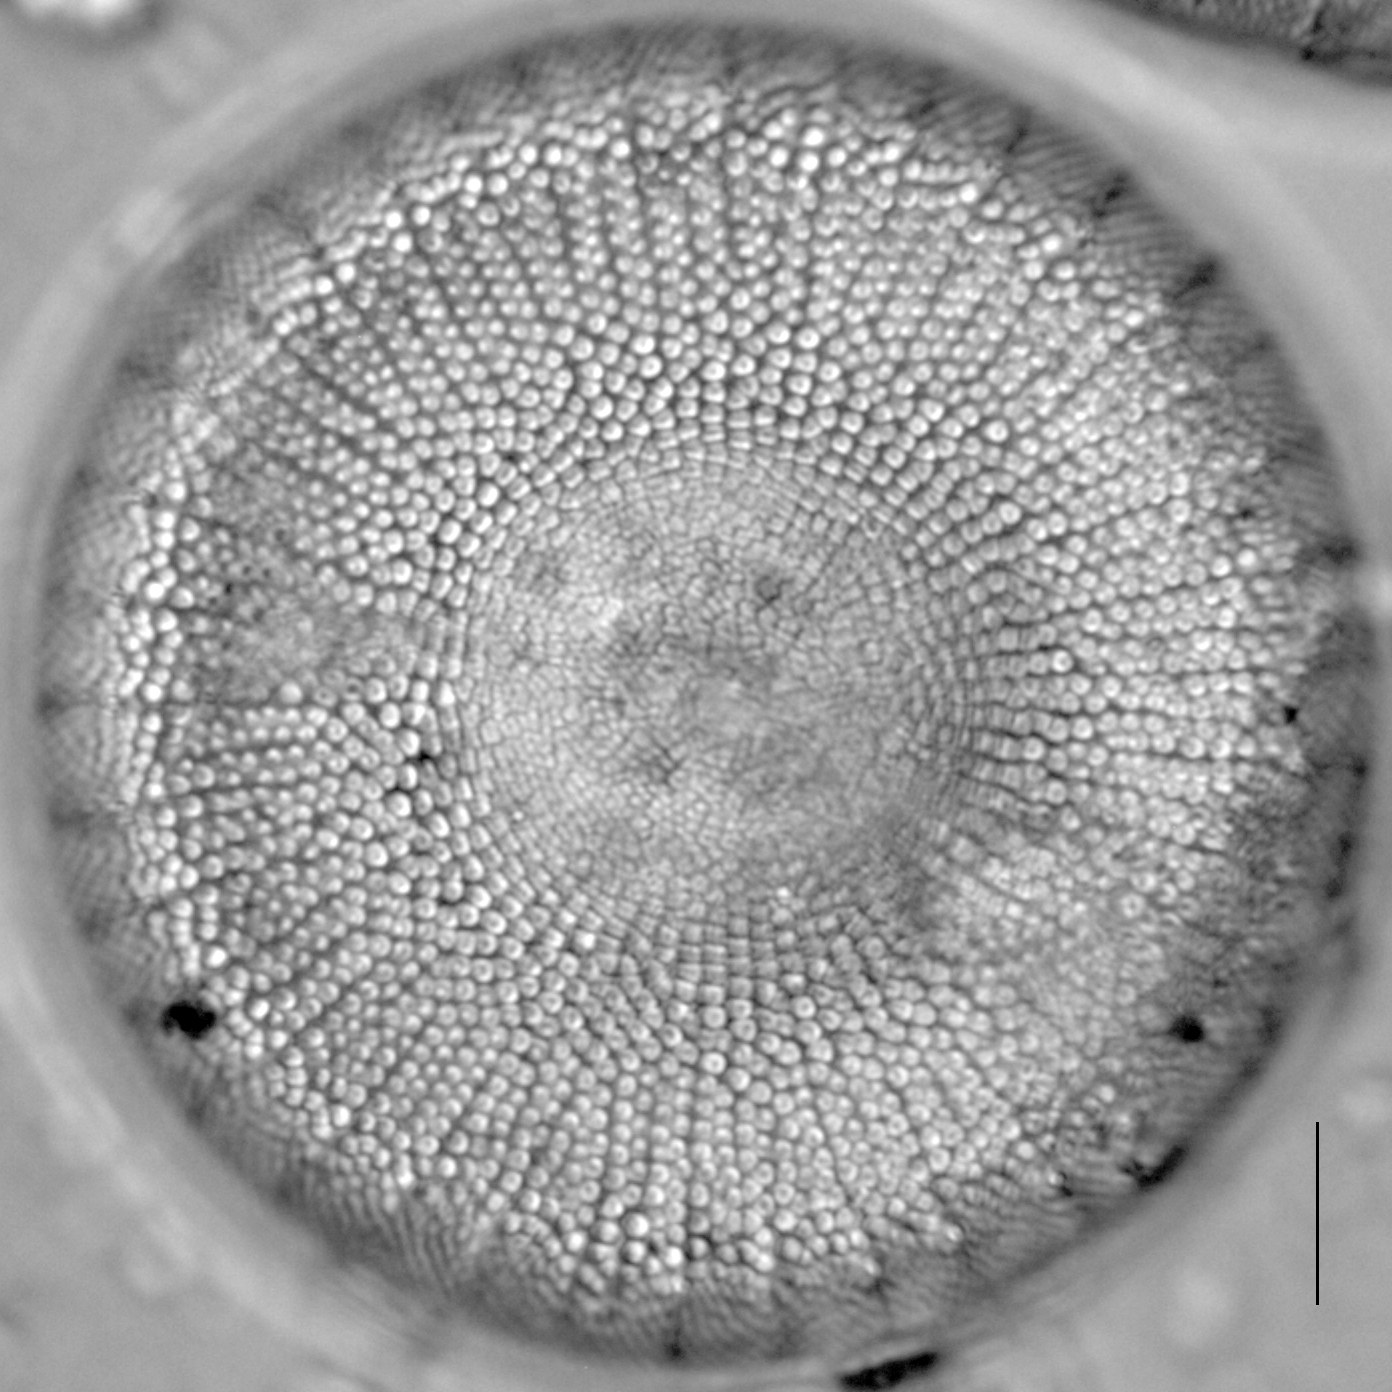
\includegraphics[width=\textwidth, height=2.2cm]{cen2.jpeg}
        \caption*{\textbf{(d) \textit{Stephanodiscus reimeri}}} % Pie de foto vacío, pero con la etiqueta
        \label{fig:sub4}
      \end{subfigure}
      \caption{Ejemplos de diatomeas con simetrias bilateral y central. \textbf{(a-b)}Especies con simetria biletaral (pennate diatom). \textbf{(c-d)} Especies con simetria central (centric diatom). }
      \label{fig:cuatro2_subfiguras}
    \end{figure}

}


\only<7>{
%Las frustulas tienen patrones intrensicos de poros y rendijas en toda su estructura. 

\begin{figure}
  \centering
  \begin{subfigure}[b]{0.2\linewidth}
    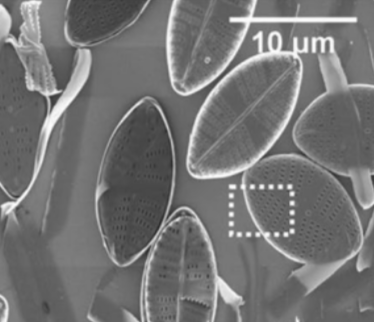
\includegraphics[width=\linewidth]{Frustrulespictures/Screen Shot 2023-07-02 at 8.24.59 PM.png} % Renombra tu archivo a este
    \caption*{\textbf{(a)}}
    \label{fig7:a}
    %\vspace{0.1cm}
  \end{subfigure}\hspace{0.5cm} % Espacio horizontal de 0.5cm
  \begin{subfigure}[b]{0.2\linewidth}
    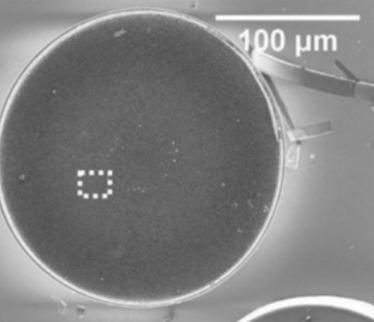
\includegraphics[width=\linewidth]{Frustrulespictures/Screen Shot 2023-07-02 at 8.25.32 PM.png} % Renombra tu archivo a este
    \caption*{\textbf{(b)}}
    \label{fig7:b}
    %\vspace{0.2cm}
  \end{subfigure}

  \begin{subfigure}[b]{0.2\linewidth}
    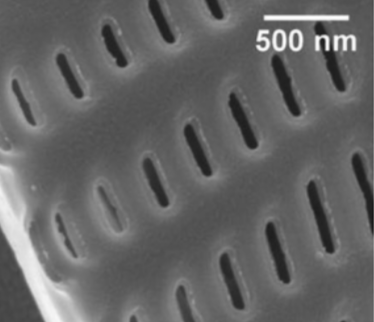
\includegraphics[width=\linewidth]{Frustrulespictures/Screen Shot 2023-07-02 at 8.25.17 PM.png} % Renombra tu archivo a este
    \caption*{\textbf{(c)}}
    \label{fig7:c}
  \end{subfigure}\hspace{0.5cm} % Espacio horizontal de 0.5cm
  \begin{subfigure}[b]{0.2\linewidth}
    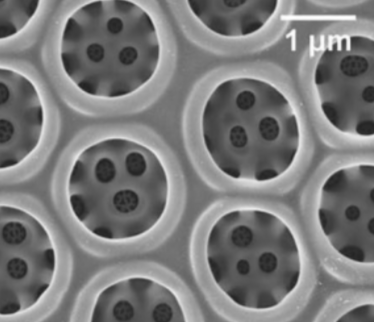
\includegraphics[width=\linewidth]{Frustrulespictures/Screen Shot 2023-07-02 at 8.25.43 PM.png} % Renombra tu archivo a este
    \caption*{\textbf{(d)}}
    \label{fig7:d}
  \end{subfigure}
  \caption{
Imágenes de microscopio electrónico de barrido (MEB) de (a,c) - \emph{Navicula perminuta}, (b,d) \emph{Coscinodiscus wailesii}. Los rectángulos punteados en (a–b) corresponden a las áreas magnificadas en (c–d) que exhibe la arquitectura del frústulo. Imágenes tomadas de \cite{aguirre2018diatomDNAViolet}.}
  \label{poresfrustrules}
\end{figure}}
\only<8>{\begin{block}{Propiedades de las frustulas:}
\begin{itemize}
\item Las frustulas tienen patrones intrensicos de poros y rendijas en toda su estructura. 
    \item Frústulo sintetizado a partir de ácido monosilícico
    %\item Superficie del frústulo con micro y nanoporos (poros)
    \item El frústulo proporciona potencial protección UV
    \item El frústulo proporciona protección mecánica
    \item Alta capacidad para la captación de luz
    %\item Productores significativos de oxígeno (20-25\% a nivel global)
    \item El frústulo exhibe estructuras similares a bandas fotónicas prohibidas
    \item Aplicaciones potenciales en la mejora de células solares
   % \item Más de 100,000 especies identificadas
    \item Categorizadas por la simetría del frústulo (céntricas y pennadas)
    %\item La acumulación lleva a la tierra de diatomeas
    %\item Parte esencial de la red trófica acuática
    \item El frústulo puede modificar la luz láser coherente
\end{itemize}
\end{block}

\vspace{1cm}

}


\end{frame}



\begin{frame}{Marco teórico}{Microscopio invertido}

\begin{figure}
    \centering
    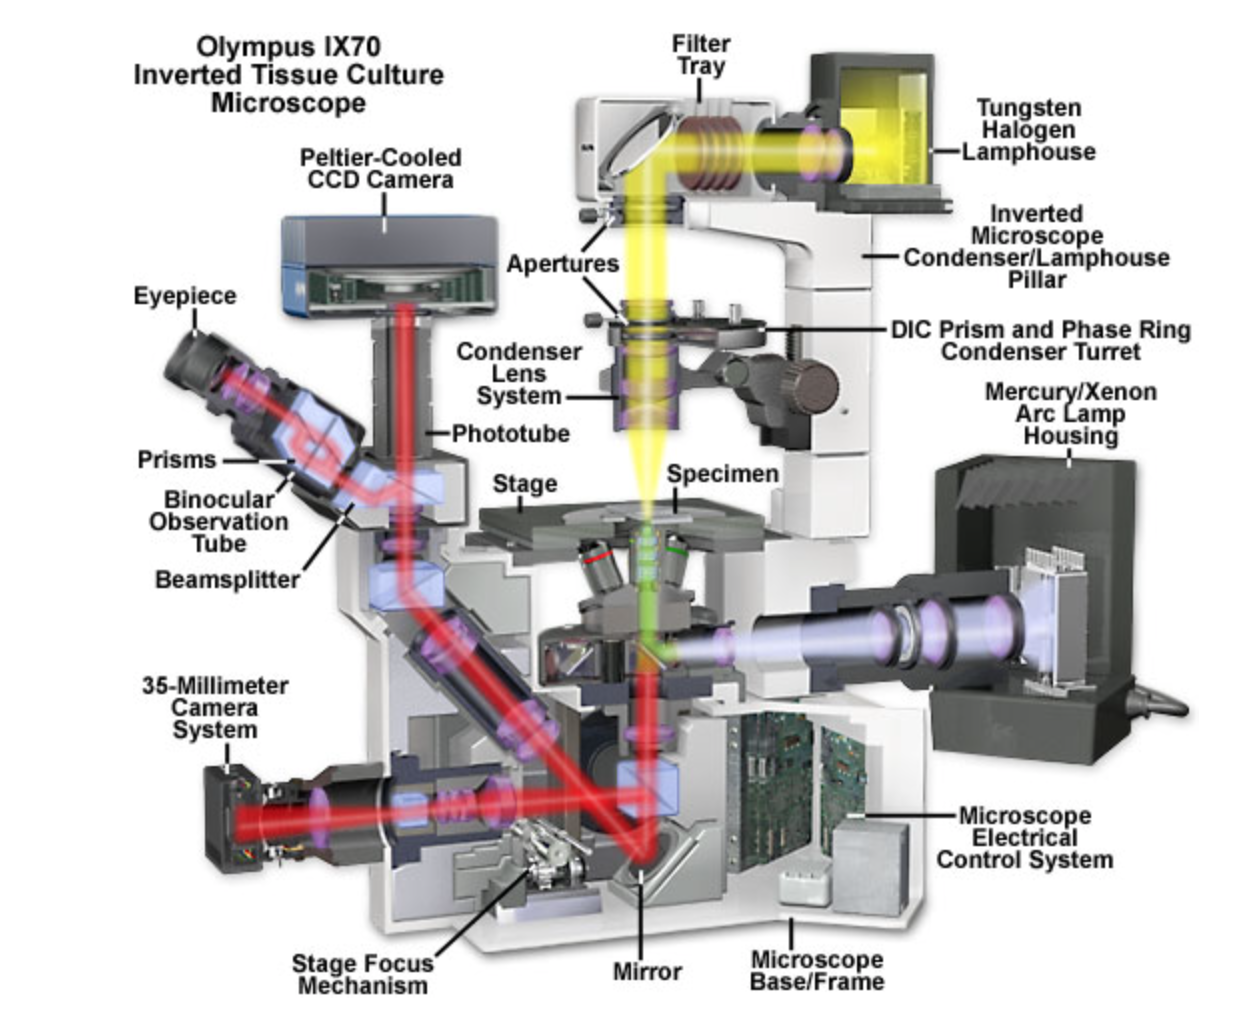
\includegraphics[scale=0.3]{Microscopeinvertedtrain.png}
    \caption{Componentes de un microscopio invertido (microscopio Olympus IX70). A diferencia de un microscopio estándar, el microscopio invertido tiene un sistema de iluminación y sus lentes de condensador por encima de la platina. Imagen tomada de \cite{Fester_Davidson_Abramowitz}. \label{FluorescenceM}}
    \label{Microscope inverted}
\end{figure}


\end{frame}
%---------------------------------
\begin{frame}<1-10>
\frametitle{Marco teórico}\framesubtitle{Pinzas opticas}
\only<1>{
Las pinzas opticas son dispositivos que permiten la manipulacion sin contacto de objetos con tamaños que varían desde la escala atómica hasta la micrométrica. 
\begin{block}{Pinzas opticas}
\begin{itemize}
\item Consisten de un haz laser altamente enfocado.
\item comunmente las pinzas opticas se generan al enfocar el haz del laser sobrellenando un lente objetivo con un alto numero de apertura. 
\item Dependiendo de la relacion entre la longitud de onda del laser y el tamano de las particulas de estudio se tienen regimenes teoricos de estudio de las fuerzas que aparecen en la presion de radiacion. 
\end{itemize}

\end{block}}
%\only<2>{\frametitle{Marco teórico}\framesubtitle{Alineacion de las pinzas opticas.}
%$M_1$}
%$M_1$ y $M_2$}

\only<2>{\frametitle{Marco teórico}
\framesubtitle{Un modelo simple.}


\begin{figure}
    \centering
    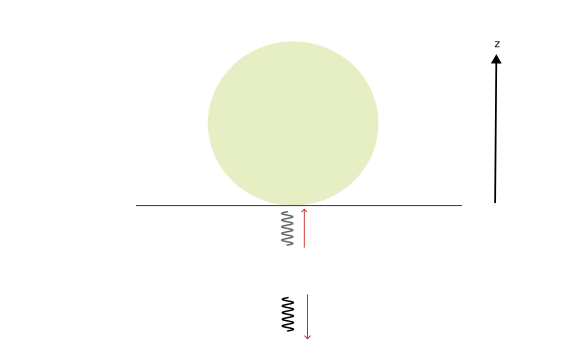
\includegraphics[scale=0.45]{foton2.png}
    \caption{Un foton con momento $\vec{p} = \frac{h}{\lambda} \hat{z}$ incide perpendicularmente en particula que funciona como un espejo perfecto.}
    \label{foton}
\end{figure}

}


\only<3>{\framesubtitle{Regimenes teoricos.}

El regimen teorico para aproximar el estudio de las fuerzas opticas en las pinzas opticas es determinado por
\begin{equation}
\xi = \frac{2\pi a n_i}{\lambda_0}
\end{equation} 
\vspace{0.8cm}
donde,
\begin{itemize}
    \item $\xi$ se define como el parámetro de tamaño de la partícula,
    \item $a$ es un parámetro característico para el tamaño de la partícula.
    \item $\lambda_0$ representa la longitud de onda de la fuente de luz en el vacío, y
    \item $n_i$ el índice de refracción del medio circundante.
\end{itemize}
}
\only<4>{
\begin{itemize}
\item Si $\xi \gg 1 $ el regimen de la optica geometrica es un buen aproximador
\item $\xi \ll 1$ Un tratamiento desde el punto de vista electromagnetico (Rayleigh), considerando a la particula atrapada como un dipolo electrico inducido oscilante. 
\item Si $\xi \sim 1$ el regimen intermedio de la teoria generalizada de Lorenz-mie es mas adecuado para describir a las fuerzas en las pinzas opticas. 

\end{itemize}\vspace{0.8 cm}
En el caso de una particula esferica de 10 micrometros de radio en agua, siendo expuesta a un laser de $532 nm$ de longitud de onda, se tiene $\xi = 157.08 \gg 1$ .
}



\only<5>{

\begin{figure}
    \centering
    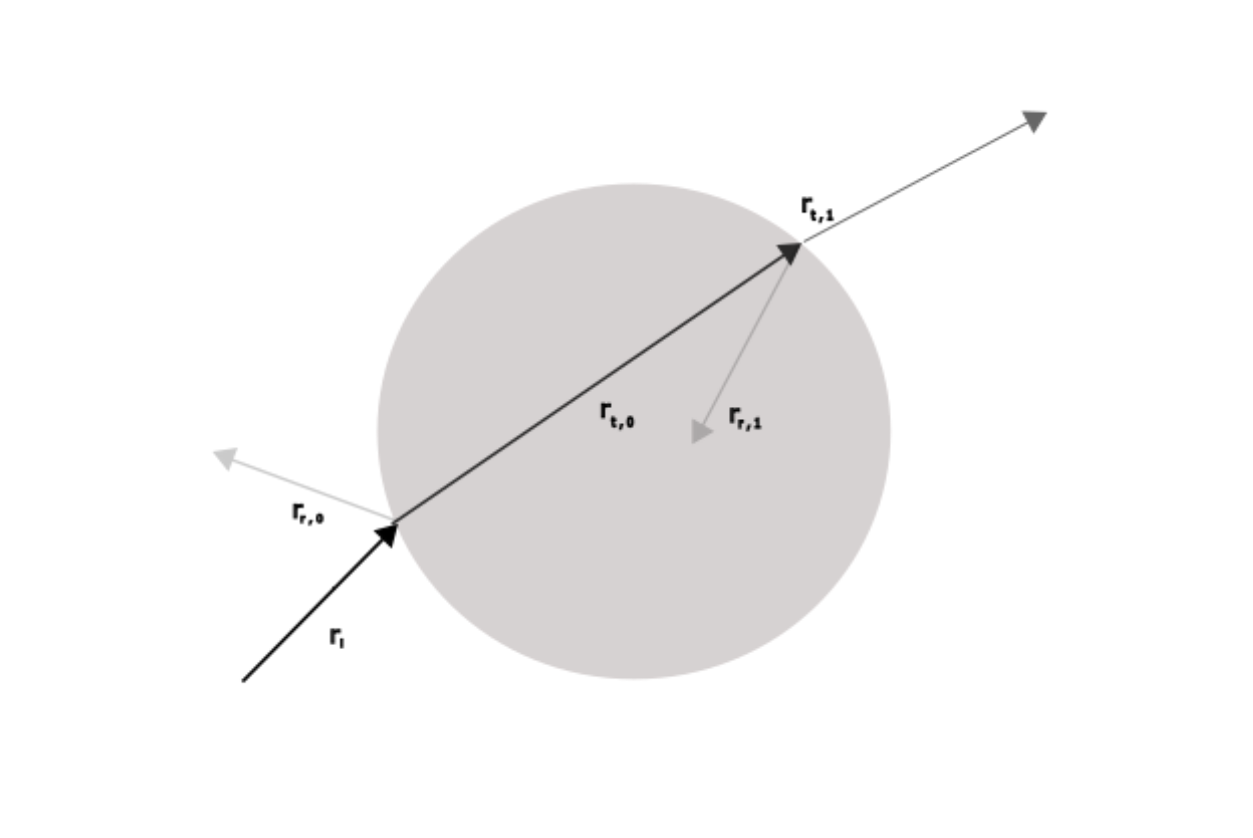
\includegraphics[scale=0.16]{beadrayoptics2.png}
    \caption{(a) Un rayo incidente $r_i$ incide sobre la superficie de una esfera. De esta interacción de dispersión, tendremos un componente transmitido y uno reflejado ($r_{r,0}$ y $r_{t,0}$) del rayo de luz. El rayo transmitido $r_{t,0}$ sufrirá otro proceso de dispersión, produciendo un nuevo par de haces de rayos ($r_{t,1}$ y $r_{r,1}$); el proceso de dispersión dentro de la esfera continuará hasta que toda la luz haya escapado de la esfera. Virtualmente toda la luz ha escapado de la esfera en menos de 10 eventos de dispersión \cite{jones2015optical}.}
    \label{bead_optics}
\end{figure}
}



\only<6>{

\begin{figure}
    \centering
    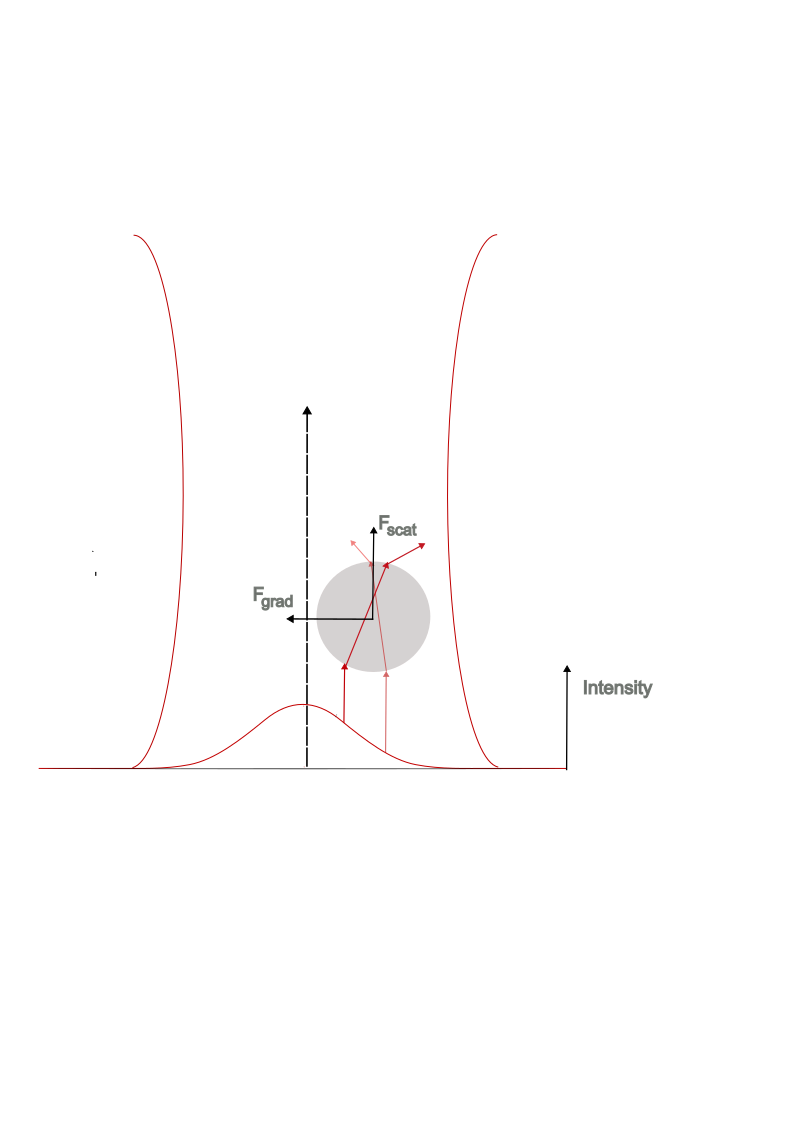
\includegraphics[trim={0cm 7.5cm 2cm 6cm },scale=0.37]{Imagenes teoria/Optical tweezer diagrams/finallyopticaltweezer.png}
    \caption{Una particula esferica sometida a un haz láser gaussiano. La esfera está fuera del eje de simetría del haz láser. Por lo tanto, la fuerza producida por el rayo de la izquierda será más fuerte que la del rayo de la derecha debido a un mayor número de fotones (mayor intensidad láser) para el primero. La figura muestra las fuerzas que actúan sobre la esfera debido al haz láser $F_{grad}$ y $F_{scat}$. }
    \label{Microscope inverted}
\end{figure}




}
\only<7>{\framesubtitle{Fuerza del primer evento de dispersion.}
Para un rayo incidente como el mostrado en la figura \ref{bead_optics}, en su primer proceso de dispersion se tiene
\begin{equation}
\mathbf{F}_{\text {ray }, 0}=\frac{n_{\mathrm{i}} P_{\mathrm{i}}}{c} \hat{\mathbf{r}}_{\mathrm{i}}-\frac{n_{\mathrm{i}} P_{\mathrm{r}}}{c} \hat{\mathbf{r}}_{\mathrm{r}}-\frac{n_{\mathrm{t}} P_{\mathrm{t}}}{c} \hat{\mathbf{r}}_{\mathrm{t}},
\label{forcefirstevent}
\end{equation}

\begin{itemize}
    \item $P_r$, $P_t$, y $P_i$ son las potencias del componente reflejado, transmitido e incidente del proceso de dispersion,
    \item $n_i$ y $n_t$ denotan los índices de refracción del medio, y la partícula respectivamente.
    \item Aquí, $\hat{\mathbf{r_i}}$, $\hat{\mathbf{r_r}}$, y $\hat{\mathbf{r_t}}$ son los vectores unitarios que representan la dirección de los componentes incidente, reflejado y transmitido para el primer proceso de dispersión del rayo de luz incidente en la esfera.
\end{itemize}
}



\only<8>{\framesubtitle{El proceso asintotico por rayo.}
De manera teorica para este rayo incidente, se tendran infinitos procesos de dispersion,
\begin{equation}
\mathbf{F}_{\text {ray }}=\frac{n_{\mathrm{i}} P_{\mathrm{i}}}{c} \hat{\mathbf{r}}_{\mathrm{i}}-\frac{n_{\mathrm{i}} P_{\mathrm{r}}}{c} \hat{\mathbf{r}}_{\mathrm{r}, 0}-\sum_{n=1}^{+\infty} \frac{n_{\mathrm{i}} P_{\mathrm{t}, n}}{c} \hat{\mathbf{r}}_{\mathrm{t}, n},
\label{infinitesum}
\end{equation}
En principio se tendria que calcular la suma infinita para encontrar la fuerza exacta, sin embargo la contribucion mas grande proviene de los dos primeros procesos y virtualmente la potencia se vuelve cero despues de las 10 iteraciones del proceso.


}
\only<9>{\framesubtitle{La fuerza total}

La fuerza total debido al la radiacion electromagnetica, considerando "todos" los rayos del haz laser. 


\begin{equation}
\mathbf{F}_{\mathrm{total}}=\sum_m \mathbf{F}_{\mathrm{ray}}^{(m)}=\sum_m\left[\frac{n_{\mathrm{i}} P_{\mathrm{i}}^{(m)}}{c} \hat{\mathbf{r}}_{\mathrm{i}}^{(m)}-\frac{n_{\mathrm{i}} P_{\mathrm{r}}^{(m)}}{c} \hat{\mathbf{r}}_{\mathrm{r}, 0}^{(m)}-\sum_{n=1}^{+\infty} \frac{n_{\mathrm{i}} P_{\mathrm{t}, n}^{(m)}}{c} \hat{\mathbf{r}}_{\mathrm{t}, n}^{(m)}\right]. 
\label{Ftotal}
\end{equation}


}
\only<10>{

\begin{figure}
    \centering
    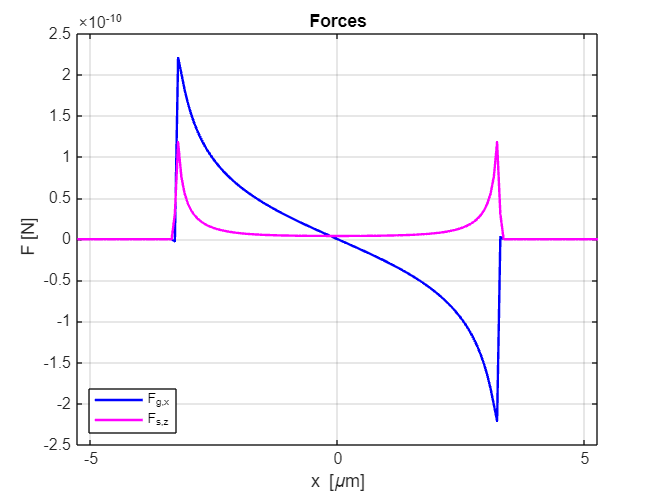
\includegraphics[scale=0.35]{Screenshot 2025-03-05 004832.png}
    \caption{Fuerzas ópticas $F_g$ y $F_s$ (fuerza de gradiente y fuerza de dispersión respectivamente) sobre una partícula esférica de $SiO_2$ de $6.59 \mu m$ producidas por un haz láser enfocado con una potencia establecida en $120 mW$. Las fuerzas ópticas se calculan en función de la posición a lo largo del eje transversal x del centro de masa de la partícula atrapada utilizando el software OTGO. El foco del haz láser en el software se considera obtenido sobrellenando un objetivo de microscopio con apertura numérica 1.0 y aumento de 60X.}
    \label{OpticalforcessetupKaren}
\end{figure} 

}


%\%begin{figure}
  %  \centering
   % 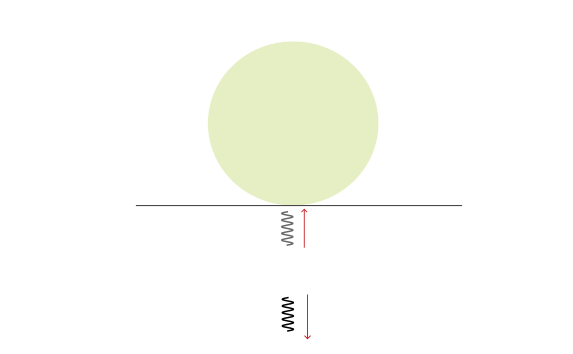
\includegraphics[scale=0.3]{foton.png}
 %   \caption{Un foton incide perpendicularmente en particula que funciona como un espejo perfecto.}
  %  \label{foton}
%\end{figure}


%}

\end{frame}



\begin{frame}<1-5>
\frametitle{Marco teorico}
\only<1>{\frametitle{Marco teorico}\framesubtitle{Microfluidicos}
Un dispositivo microfluídico es un sistema diseñado para manipular y manejar pequeñas cantidades de fluidos a escala de micrómetros.
 \begin{figure}
     \centering
     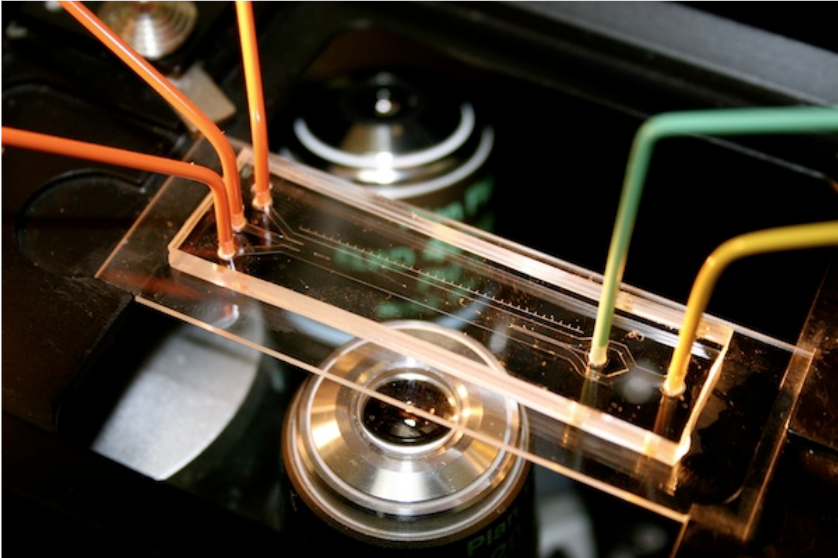
\includegraphics[scale=0.35]{microfluidicinaction.png}
     \caption{Un dispositivo microfluídico colocado en la platina de un microscopio invertido. Esta configuración permite el seguimiento visual de los fenómenos que ocurren en los microcanales. Imagen tomada de \cite{Wanucha_2012} con permiso de los autores.}
     \label{microfluidic_device} .
 \end{figure}}
 
 \only<2>{\framesubtitle{Microfluidicos: Un diseño simple.}
 
 \begin{figure}
     \centering
     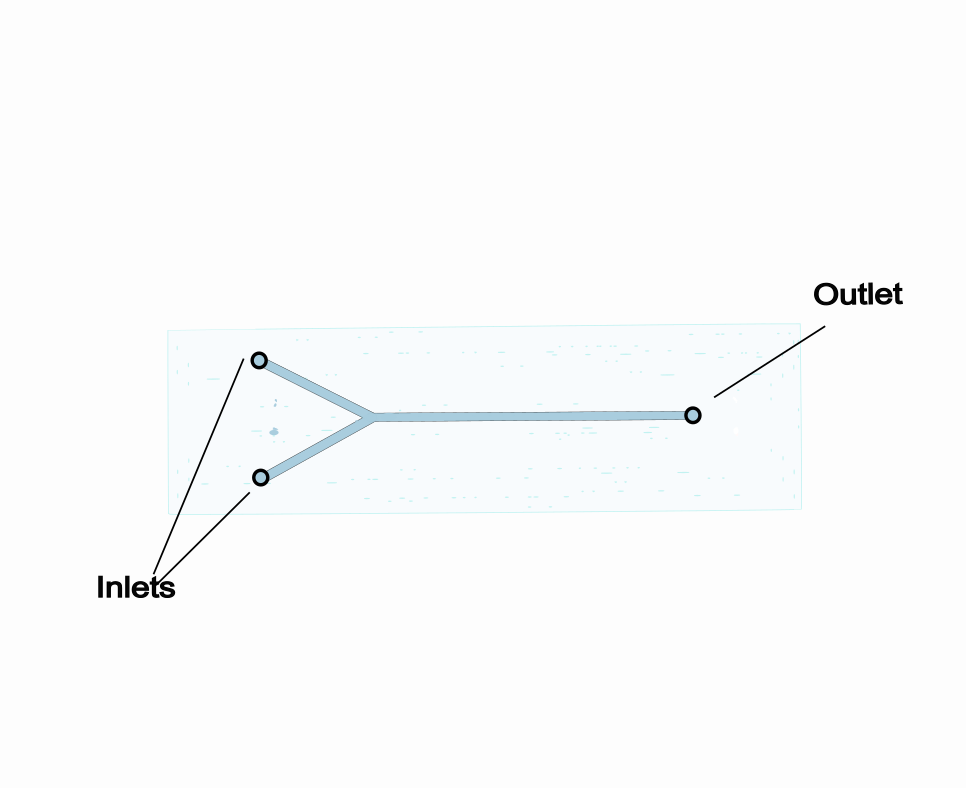
\includegraphics[trim = {0 1.5cm 0 0.7cm}, scale=0.4]{Diatomsexperimentalmethods/Microfluidics designs/Screen Shot 2024-01-17 at 5.34.18 PM.png}
     \caption{Un diseño tipo Y de dispositivo microfluídico. Con dos entradas y una salida, este diseño es útil para aplicaciones de mezcla de microfluidos y microrreactores \cite{niculescu2022review}. }
     \label{simple design}
 \end{figure}
 
 
 
 }
\only<3>{\framesubtitle{Microfluidicos: propiedades}

 \begin{block}{Propiedades de los microfluidicos}
 \begin{itemize}
    \item Capacidad para manejar y manipular pequeñas cantidades de fluidos a escala de micrómetros o inferior.
    \item Red de microcanales interconectados.
    \item Control preciso del flujo del líquido.
    \item Permite un entorno estable para experimentos donde se requiere regulación estricta de temperatura, presión y concentraciones químicas.
    \item Proporciona un flujo continuo de fluido y recarga en caso de evaporación o intercambio de fluidos.
   % \item Permite la aceleración del fluido y la manipulación controlada.
    \item Fabricación con diversos materiales (silicio, vidrio, PDMS, metales), ofreciendo diversas propiedades físicas.
    \item Variedad de diseños para la red de canales.
    \item Bajo consumo de muestra.
\end{itemize}
 \end{block}
 
 }
 \only<4>{\framesubtitle{Utilidad de los microfluidicos}
 
 
 Los dispositivos microfluídicos encuentran aplicaciones en un amplio espectro de campos, incluyendo la biología (p. ej., análisis de ADN y clasificación celular \cite{wang2011enhancedmicroandopti,paegel2003microfluidicDNA}), la química (p. ej., síntesis y análisis de químicos \cite{niculescu2022review}) y la física (p. ej., estudios de dinámica de fluidos).}
 
 \only<5>{\framesubtitle{La fuerza de Stokes}

Para una partícula esférica de radio \( r \) que se mueve con una velocidad \( \mathbf{v} \) en un fluido de viscosidad dinámica \( \mu \), la fuerza de arrastre \( \mathbf{F}_d \) es
\begin{equation}
    \mathbf{F}_d = 6 \pi \mu r \mathbf{v}.
\end{equation} 
 
 }
 
\end{frame}

\section{Metodos experimentales}
\begin{frame}{Metodos experimentales}{Arreglo experimental}

\begin{figure}
    \centering
    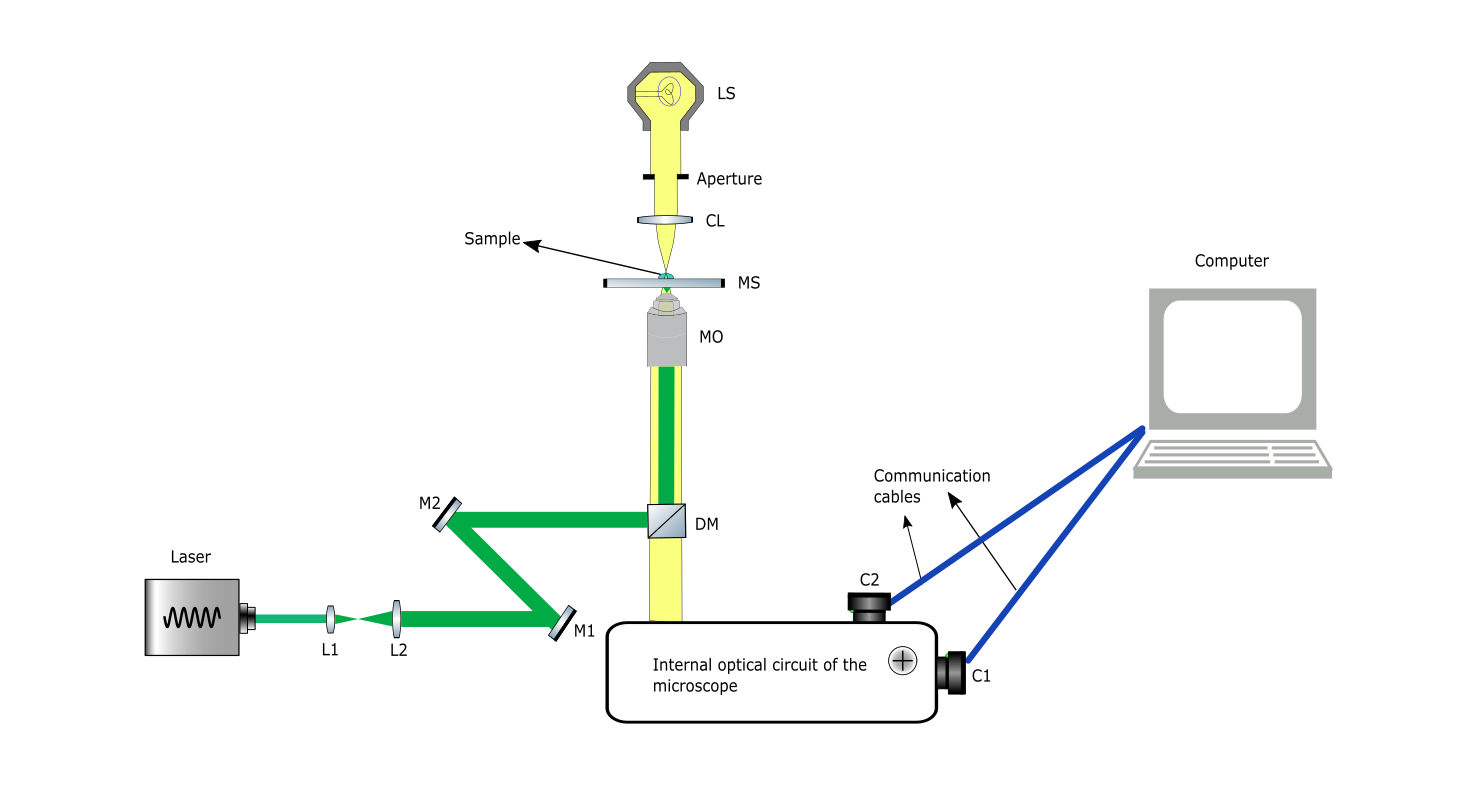
\includegraphics[scale=0.27]{Newplots_microfluidics_results/setup3.png}
    \caption{Configuración estándar para pinzas ópticas. Un dispositivo láser facilita la radiación para producir la trampa óptica. $L_1$ y $L_2$ son dos lentes positivas. Estas lentes se colocan a una distancia $f_1 + f_2$ entre sí, expandiendo el haz láser para sobrellenar la apertura trasera del objetivo del microscopio (MO). $M_1$ y $M_2$ son espejos para alinear el haz láser. La luz láser es reflejada hacia la apertura trasera del objetivo del microscopio (MO) por un espejo dicróico (DM).}
    \label{setuptweezers}
\end{figure}

\end{frame}



\begin{frame}{Metodos experimentales}{Alineacion de las pinzas opticas.}
\begin{figure}[H]
    \centering
    \subfloat[\centering]{{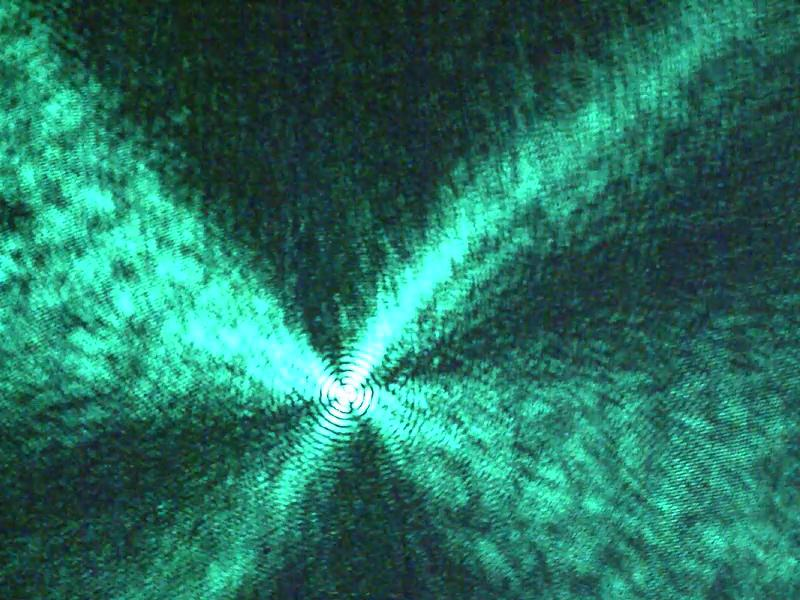
\includegraphics[scale=0.12]{Diatomsexperimentalmethods/Backscateringpattern/backscattered.jpeg} }}%
    \qquad
    \subfloat[\centering]{{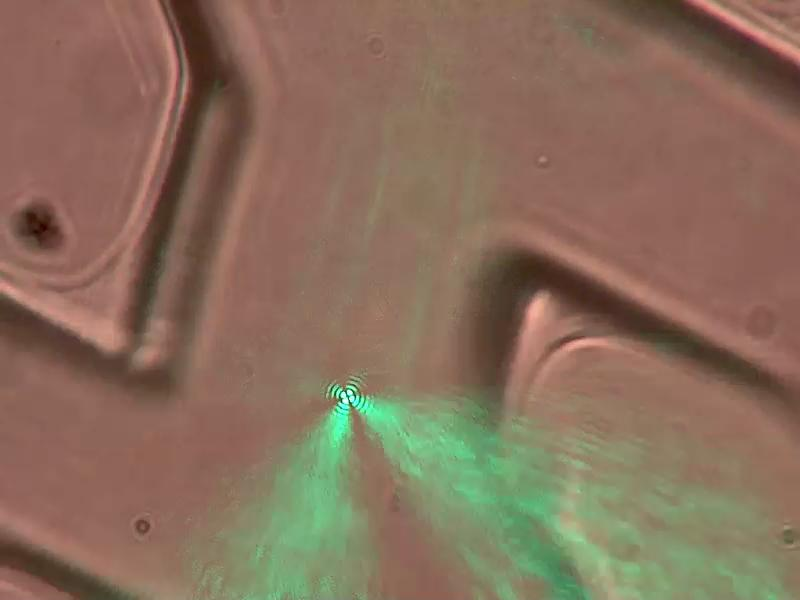
\includegraphics[scale=0.12]{Diatomsexperimentalmethods/Backscateringpattern/inmicrofluidics.jpeg} }}%
    \caption{Patrones de luz retrodispersada capturados con la cámara Axis M1103. En ambas figuras se utilizó el objetivo de microscopio de inmersión en agua para enfocar la luz láser. (a) Patrón de radiación retrodispersada producido desde un portaobjetos sin muestra. (b) Patrón de radiación retrodispersada observado a través del dispositivo microfluídico utilizado en este trabajo.}%
    \label{symmetricpattern}%
\end{figure}
\end{frame}

\begin{frame}{Metodos experimentales}{Especificos}

\end{frame}

\begin{frame}<1-4>\frametitle{Metodos experimentales}\framesubtitle{Muestras}

\only<1>{
\begin{itemize}
\item Las particulas de $SiO_2$ artificiales utilizadas ($24.82 \mu m$, $19.98 \mu m$, $6.59 \mu m$, y $4.27 \mu m$) estaban contenidas en una suspension acuosa con concentracion de $2.5 \% w/v$.
\item Solución acuosa de células de levadura al $2\%$ $p/v$ (peso/volumen).
\item Las especies de diatomeas utilizadas son \textit{Nitzschia sp}, \textit{Phaeodactylum tricornutum}, \textit{Thalassiosira pseudonana}, \textit{Navicula Sp. 12} y  \textit{Marine pennate}.
\end{itemize}




}


\only<2>{

\begin{figure} [H]
\centering
\begin{tabular}{ccc}
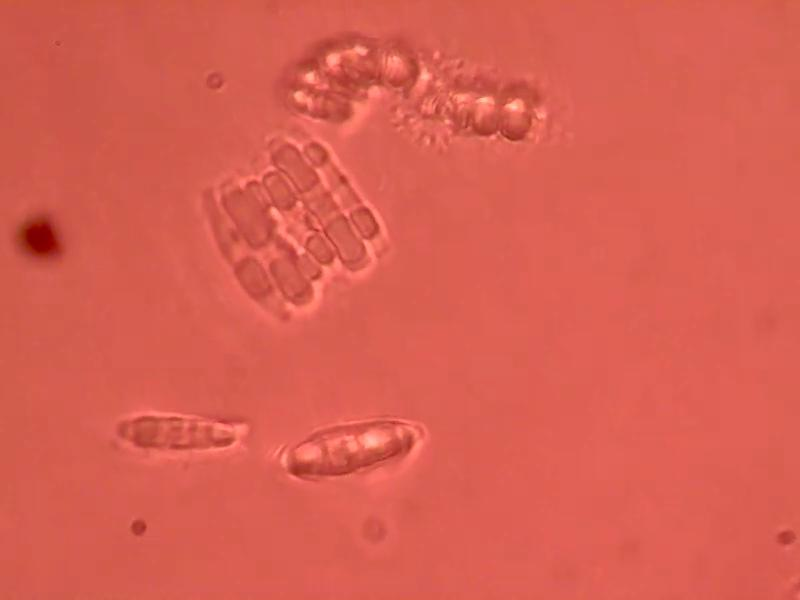
\includegraphics[width=0.22\textwidth]{Diatomsexperimentalmethods/Nitzchia sp1.jpeg} &
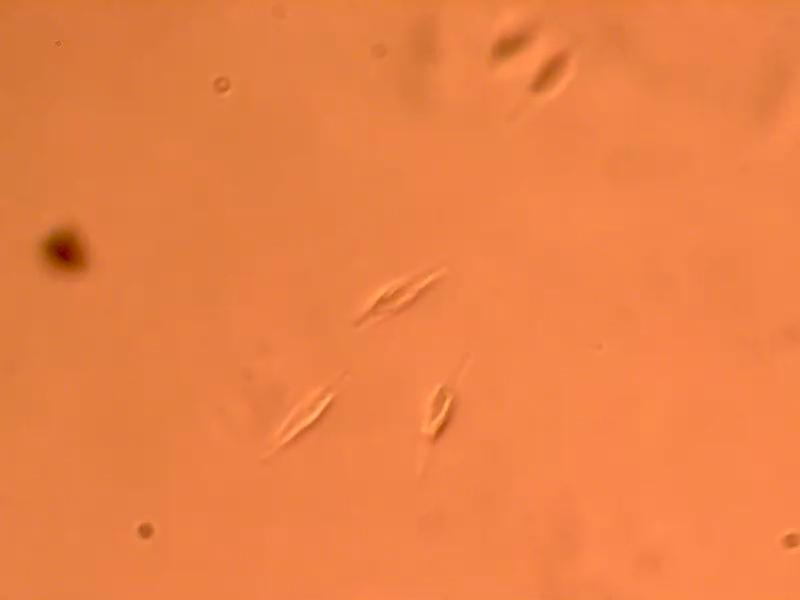
\includegraphics[width=0.22\textwidth]{Diatomsexperimentalmethods/Phaeodactylum t.jpgss.jpg} &
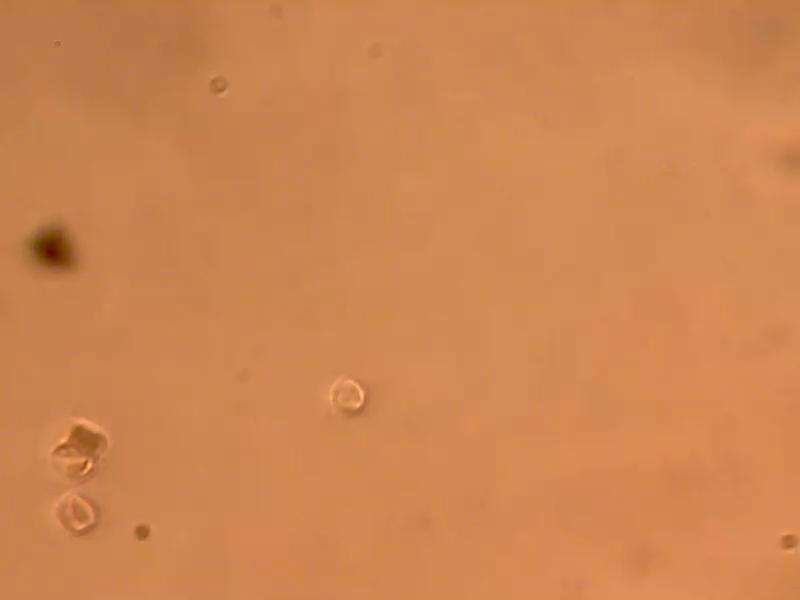
\includegraphics[width=0.22\textwidth]{Diatomsexperimentalmethods/thala2.jpeg} \\
\text{(a)}  & \text{(b)} & \text{(c)}  \\[6pt]
\end{tabular}

\vspace{6pt}

\begin{tabular}{cc}
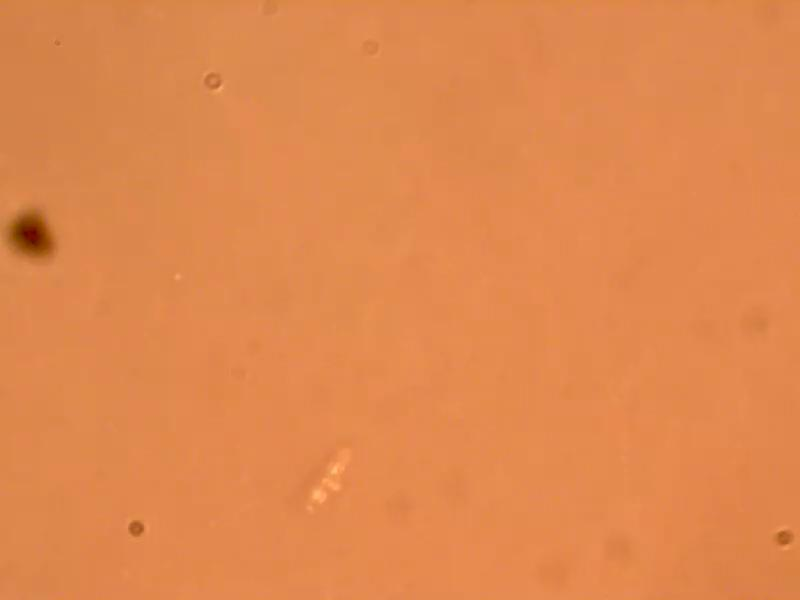
\includegraphics[width=0.22\textwidth]{Diatomsexperimentalmethods/gea4al.jpeg} &
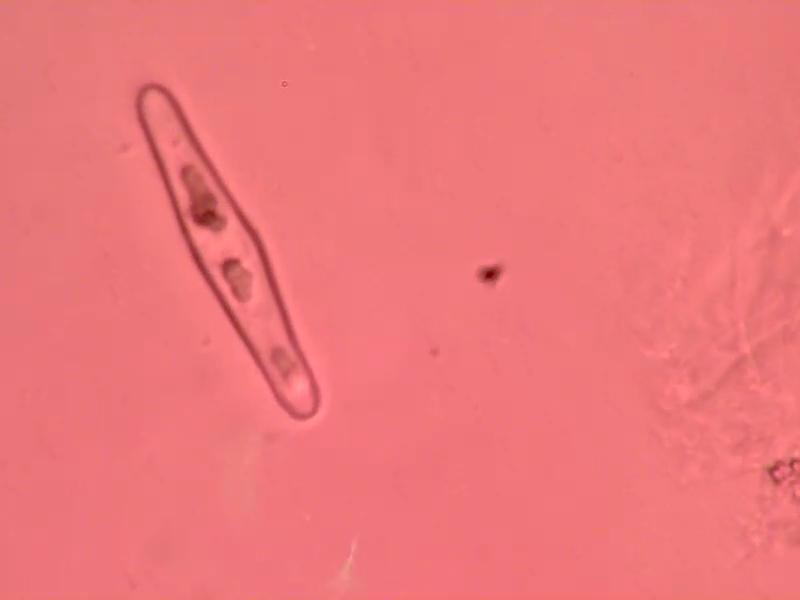
\includegraphics[width=0.22\textwidth]{Diatomsexperimentalmethods/ray.jpeg} \\
\text{(d)}  & \text{(e)}  \\[6pt]
\end{tabular}
\caption{Especies de diatomeas estudiadas en este trabajo, fotografiadas con el objetivo de microscopio de inmersión en agua. (a) Multitud de \textit{Nitzschia sp}. (b) Muestra de la especie de diatomea \textit{Phaeodactylum tricornutum}. (c) Muestra de la especie de diatomea \textit{Thalassiosira pseudonana}. (d) Diatomea \textit{Navicula Sp. 12}. (e) Diatomea \textit{Pennada marina}}.
\label{DiatomExperiments}
\end{figure}



}

\only<3>{\framesubtitle{Preparacion de muestras}

\begin{figure}
    \centering
    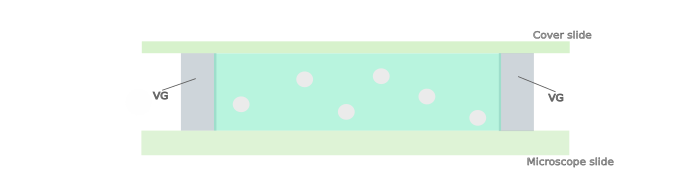
\includegraphics[trim ={1cm 0 0cm 0cm}, scale=.6]{Imagenes teoria/cuci.png}
    \caption{Preparación de la muestra. Una barrera de grasa de vacío (VG) contiene las suspensiones acuosas con las partículas a ser atrapadas entre el cubreobjetos y el portaobjetos.} %La muestra se coloca en la platina del microscopio para visualizar las partículas y probar la capacidad de atrapamiento de las pinzas ópticas.}% you need long time for this experiments.
    \label{VG}
\end{figure}




}
\only<4>{
\framesubtitle{Microfluidicos}
\begin{figure}[H]
    \centering
    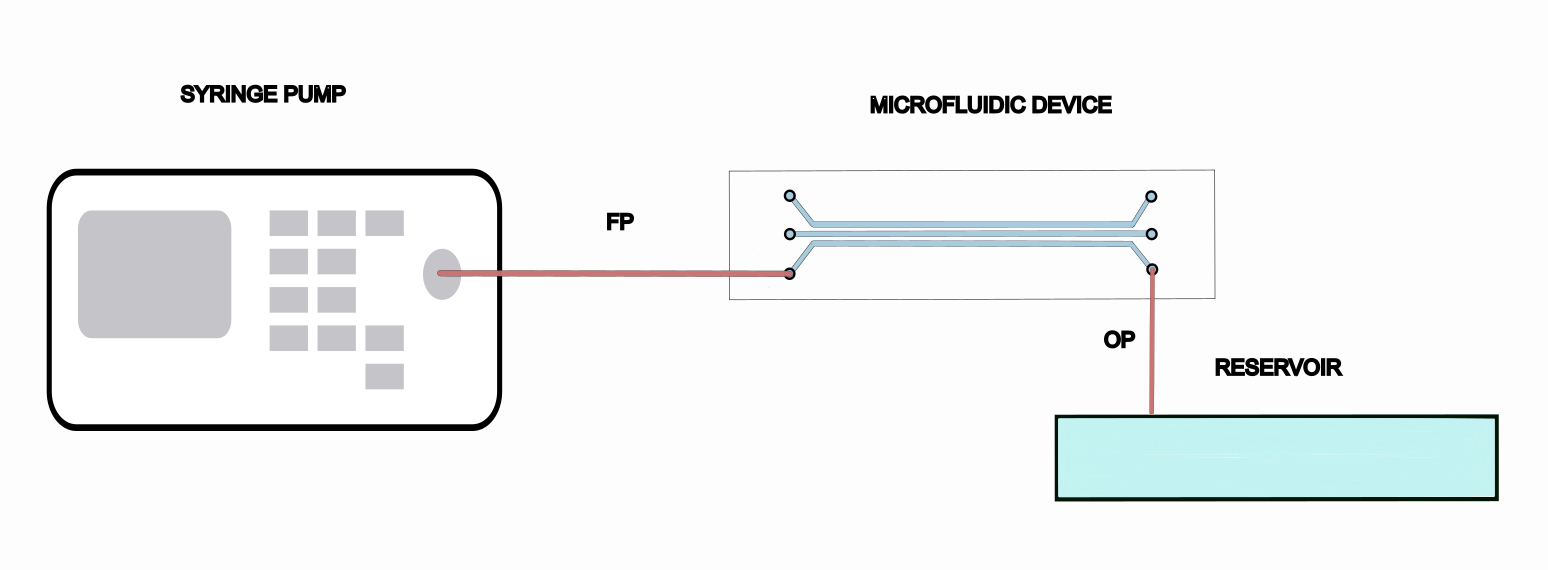
\includegraphics[scale=0.35]{Diatomsexperimentalmethods/Samplepreparation/Screen Shot 2024-01-18 at 12.50.20 PM.png}
    \caption{Esquema del sistema microfluídico. La bomba de jeringa controla la velocidad de flujo de la solución que entra al canal a través del tubo de alimentación (FP) integrado en la entrada del canal. Una vez que el fluido alcanza la salida del canal, un tubo de salida (OP) dirige la solución efluente a un reservorio.}
    \label{microfluidicsystem}
\end{figure}


}

\end{frame}



%-------------------------------------------------------
\section{Resultados}
%-------------------------------------------------------
\begin{frame}<1-3>
\frametitle{Resultados}\framesubtitle{Manipulacion de particulas de silica.}

\only<1>{
\begin{figure}
  \centering
  \begin{subfigure}[b]{0.2\linewidth}
    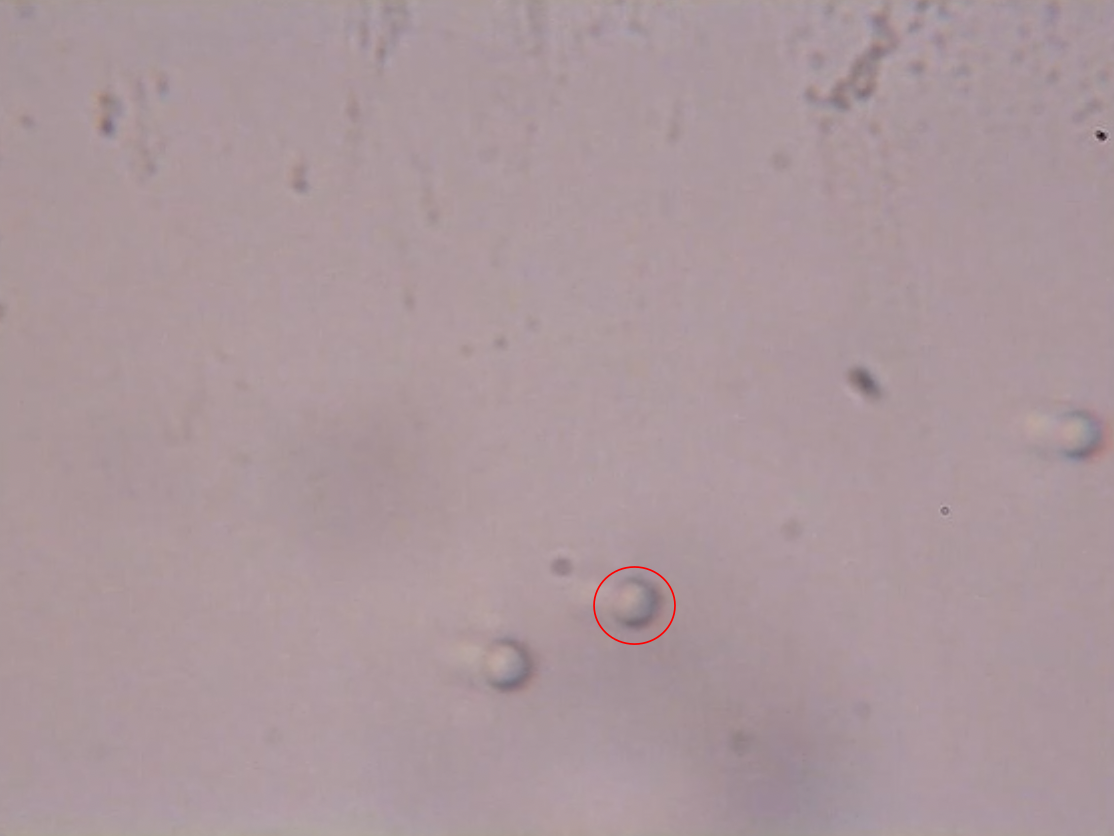
\includegraphics[width=\linewidth]{427particles/image732.png} % Renombra tu archivo a este
    \caption*{\textbf{(a)}}
    \label{fig7:a}
    %\vspace{0.1cm}
  \end{subfigure}\hspace{0.5cm} % Espacio horizontal de 0.5cm
  \begin{subfigure}[b]{0.2\linewidth}
    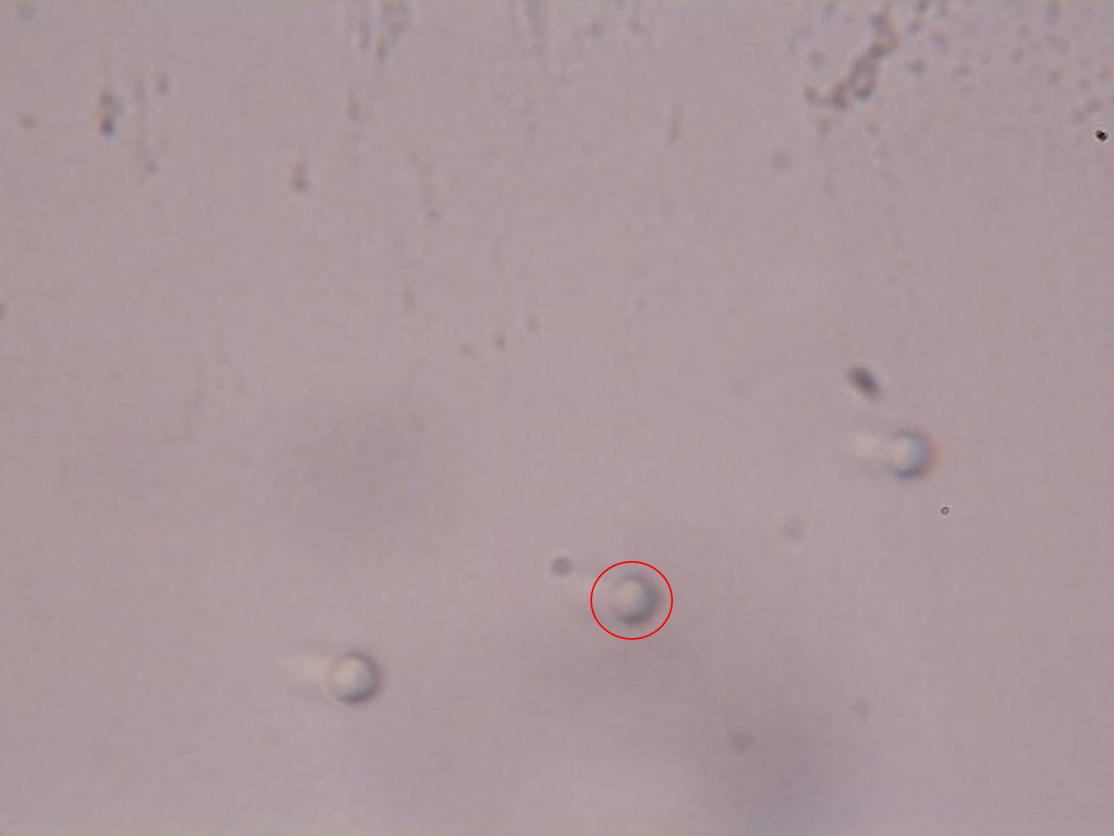
\includegraphics[width=\linewidth]{427particles/2.png} % Renombra tu archivo a este
    \caption*{\textbf{(b)}}
    \label{fig7:b}
    %\vspace{0.2cm}
  \end{subfigure}

  \begin{subfigure}[b]{0.2\linewidth}
    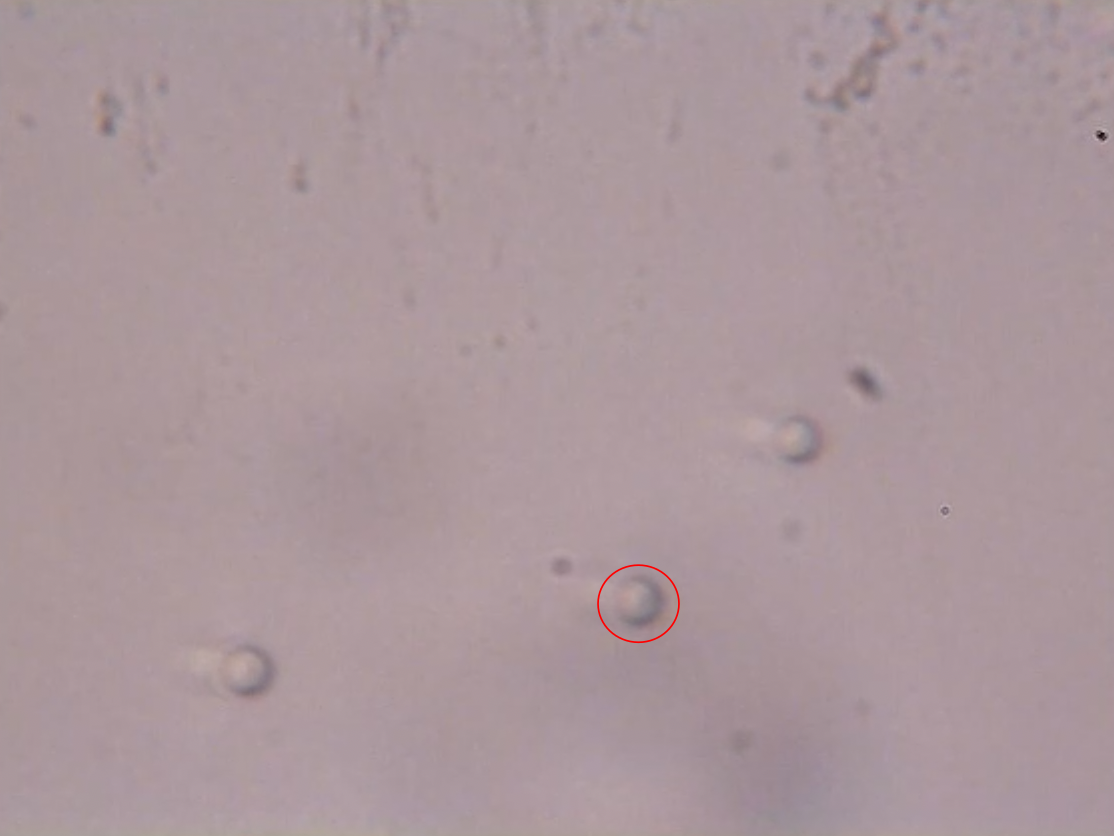
\includegraphics[width=\linewidth]{427particles/i.png} % Renombra tu archivo a este
    \caption*{\textbf{(c)}}
    \label{fig7:c}
  \end{subfigure}\hspace{0.5cm} % Espacio horizontal de 0.5cm
  \begin{subfigure}[b]{0.2\linewidth}
    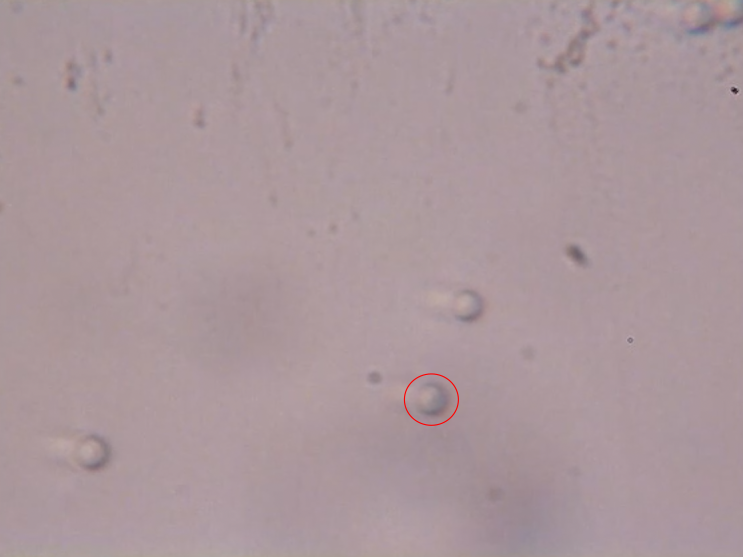
\includegraphics[width=\linewidth]{427particles/4.png} % Renombra tu archivo a este
    \caption*{\textbf{(d)}}
    \label{fig7:d}
  \end{subfigure}
  \caption{
Atrapamiento de partículas de $SiO_2$ de 4.27 $\mu m$. Potencia láser incidente establecida en 53 $mW$ llegando a la apertura trasera del objetivo de microscopio de inmersión en agua con un expansor de haz de 10x. (a-d) La partícula atrapada (círculo rojo) permanece estacionaria, mientras que las circundantes son movidas con el joystick del controlador del stage.}
  \label{poresfrustrules}
\end{figure}}


\only<2>{

\begin{figure}
    \centering
    \includemovie[autoplay]{12cm}{7cm}{circle.mp4}
    \caption{Atrapamiento de partículas de $SiO_{2}$ de $24.82 \mu m$. La trampa se produjo con el objetivo de inmersión en agua (MO) y un expansor de haz de 5x (potencia láser establecida en 96 $mW$).}
    \label{fig:enter-label}
\end{figure}


}



\only<3>{

\begin{figure}
    \centering
    \includemovie[autoplay]{12cm}{7cm}{video2.mp4}
    \caption{Atrapamiento de partículas de $SiO_{2}$ de $24.82 \mu m$. La trampa se produjo con el objetivo de inmersión en agua (MO) y un expansor de haz de 5x (potencia láser establecida en 96 $mW$).}
    \label{fig:enter-label}
\end{figure}

}
\end{frame}

\begin{frame}<1-2>
\frametitle{Resultados}\framesubtitle{Atrapamiento de celulas de levadura.}
\only<1>{

\begin{figure}
  \centering
  \begin{subfigure}[b]{0.2\linewidth}
    \includegraphics[width=\linewidth ,height=2.3cm]{particles2.png} % Renombra tu archivo a este
    \caption*{\textbf{(a)}}
    \label{fig7:a}
    %\vspace{0.1cm}
  \end{subfigure}\hspace{0.5cm} % Espacio horizontal de 0.5cm
  \begin{subfigure}[b]{0.2\linewidth}
    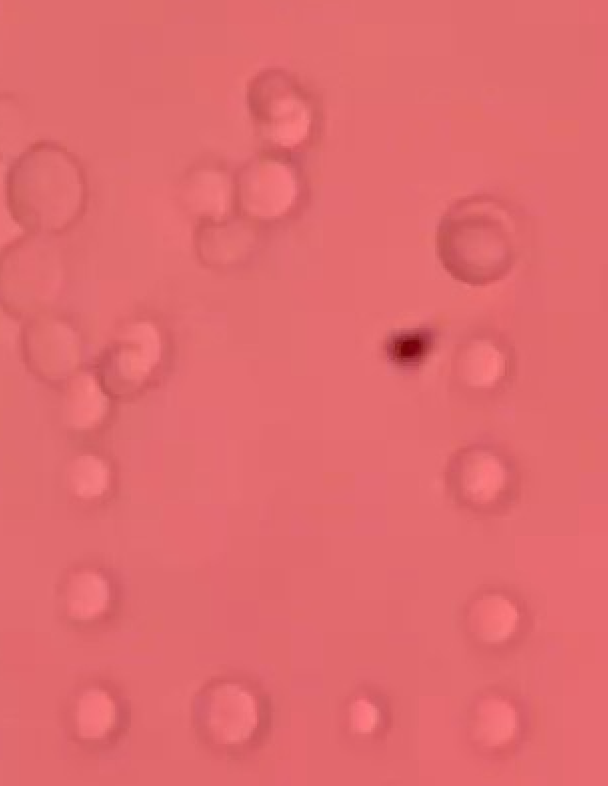
\includegraphics[width=\linewidth ,,height=2.3cm]{particles7.png} % Renombra tu archivo a este
    \caption*{\textbf{(b)}}
    \label{fig7:b}
    %\vspace{0.2cm}
  \end{subfigure}

  \begin{subfigure}[b]{0.2\linewidth}
    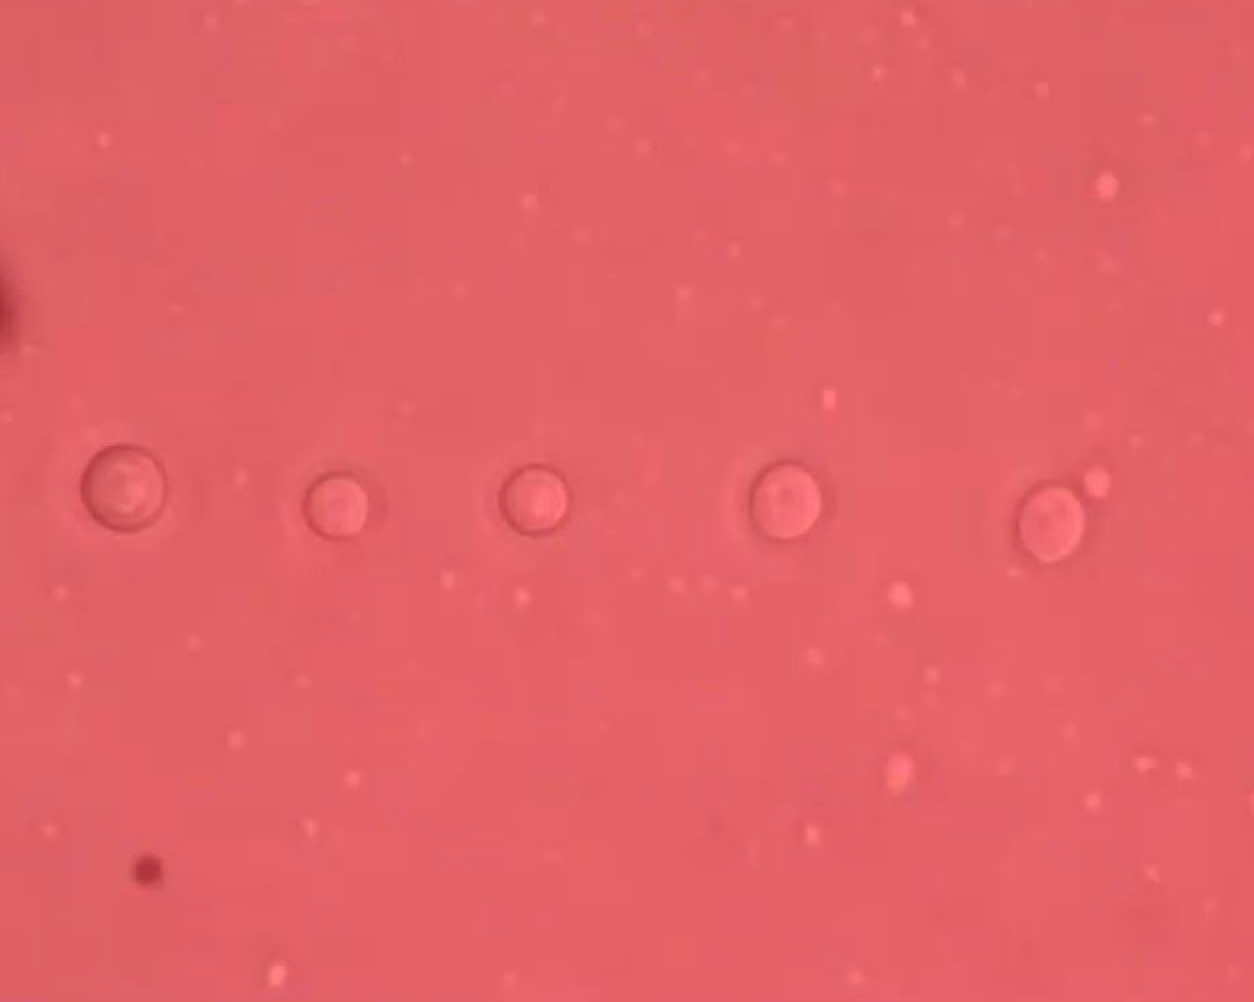
\includegraphics[width=\linewidth]{particlesnow.png} % Renombra tu archivo a este
    \caption*{\textbf{(c)}}
    \label{fig7:c}
  \end{subfigure}\hspace{0.5cm} % Espacio horizontal de 0.5cm
  \begin{subfigure}[b]{0.2\linewidth}
    \includegraphics[width=\linewidth]{Particles3.png} % Renombra tu archivo a este
    \caption*{\textbf{(d)}}
    \label{fig7:d}
  \end{subfigure}
  \caption{
Atrapamiento de partículas de $SiO_2$ de 4.27 $\mu m$. Potencia láser incidente establecida en 53 $mW$ llegando a la apertura trasera del objetivo de microscopio de inmersión en agua con un expansor de haz de 10x. (a-d) La partícula atrapada (círculo rojo) permanece estacionaria, mientras que las circundantes son movidas con el joystick del controlador del stage.}
  \label{poresfrustrules}
\end{figure}


}



\only<2>{\framesubtitle{Opticution de celula de levadura.}

\begin{figure}
     \centering
     \begin{subfigure}[b]{0.49\textwidth}
         \centering
         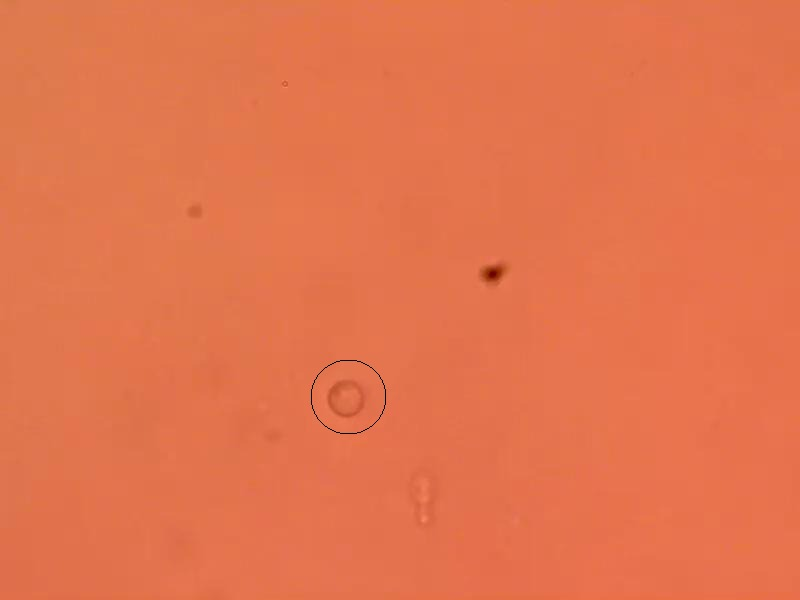
\includegraphics[width=0.50\textwidth]{Imagenes teoria/opticution0_edited.jpeg}
         \caption{Trapped yeast cell with 14 $mW$}
         \label{fig:y equals x}
     \end{subfigure}
     \hfill
     \begin{subfigure}[b]{0.49\textwidth}
         \centering
         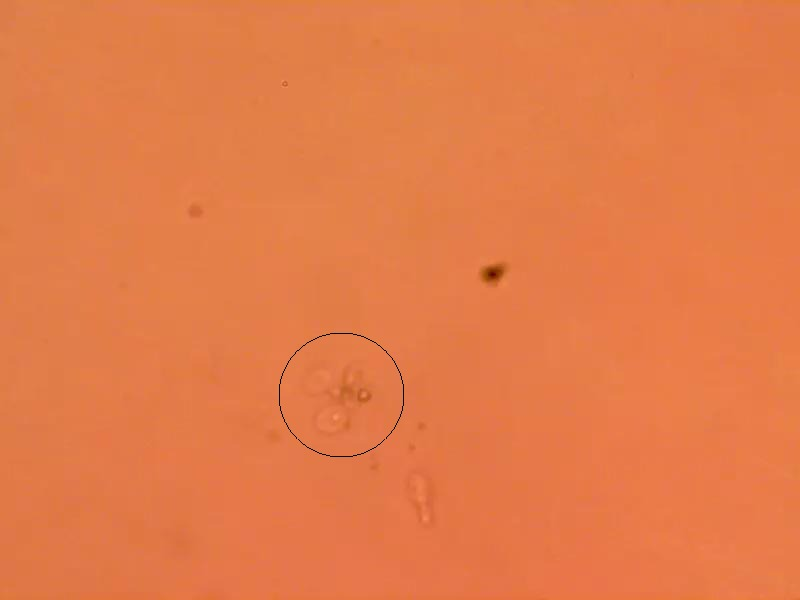
\includegraphics[width=0.50\textwidth]{Imagenes teoria/opticution1_edited.jpeg}
         \caption{Opticuted yeast cell with 695 $mW$}
         \label{fig:three sin x}
     \end{subfigure}
     
     \caption{Opticution (dead by light) of a yeast cell with a 10x beam expander, and the water immersion microscope objective.}
     \label{opticution}
     \hfill
\end{figure}

}





\end{frame}


\begin{frame}<1-5>
\frametitle{Resultados}\framesubtitle{Atrapamiento de diatomeas pennate}

\only<1>{

\begin{figure}
  \centering
  \begin{subfigure}[b]{0.2\linewidth}
    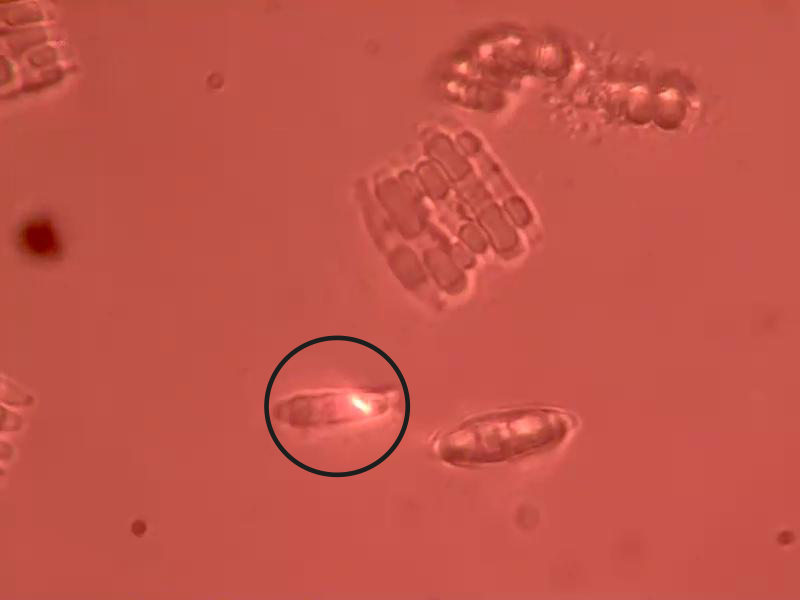
\includegraphics[width=\linewidth ,height=2.3cm]{ResultadosAlgea1/11.png} % Renombra tu archivo a este
    \caption*{\textbf{(a)}}
    \label{fig7:a}
    %\vspace{0.1cm}
  \end{subfigure}\hspace{0.5cm} % Espacio horizontal de 0.5cm
  \begin{subfigure}[b]{0.2\linewidth}
    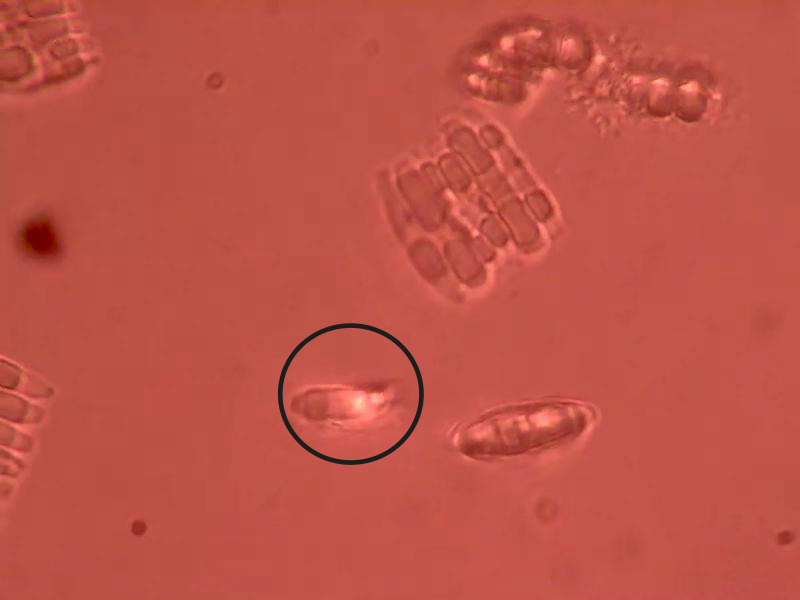
\includegraphics[width=\linewidth ,,height=2.3cm]{ResultadosAlgea1/levantando.png} % Renombra tu archivo a este
    \caption*{\textbf{(b)}}
    \label{fig7:b}
    %\vspace{0.2cm}
  \end{subfigure}

  \begin{subfigure}[b]{0.2\linewidth}
    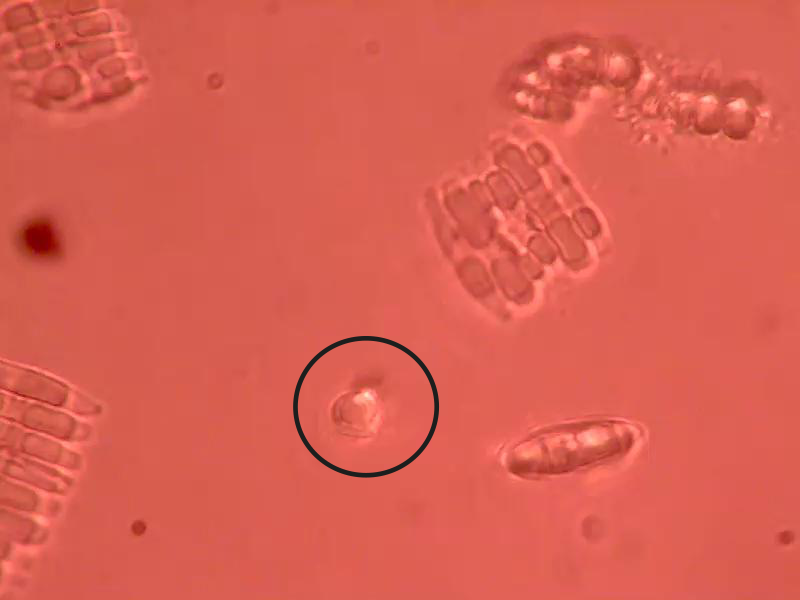
\includegraphics[width=\linewidth]{ResultadosAlgea1/3.png} % Renombra tu archivo a este
    \caption*{\textbf{(c)}}
    \label{fig7:c}
  \end{subfigure}\hspace{0.5cm} % Espacio horizontal de 0.5cm
  \begin{subfigure}[b]{0.2\linewidth}
    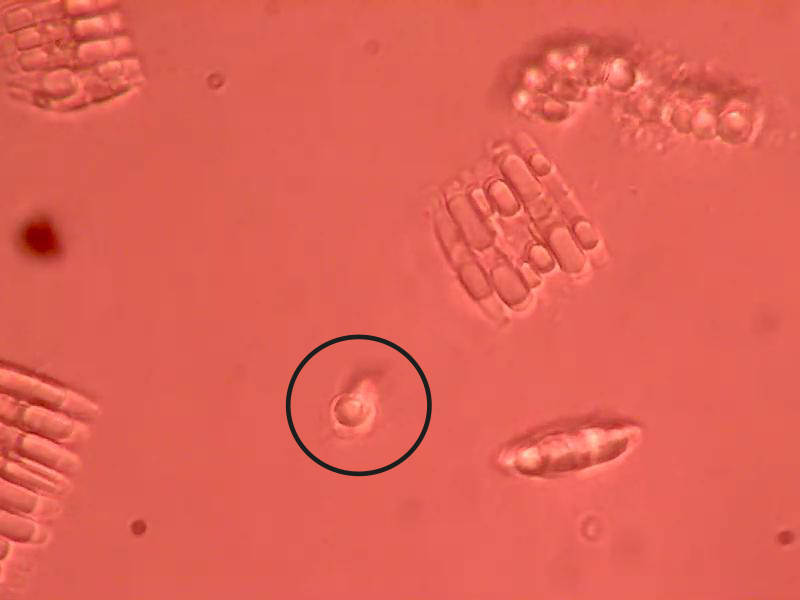
\includegraphics[width=\linewidth]{ResultadosAlgea1/1.png} % Renombra tu archivo a este
    \caption*{\textbf{(d)}}
    \label{fig7:d}
  \end{subfigure}
  \caption{
Manipulación de \textit{Nitzschia Sp.1} (pennada) con el objetivo de inmersión en agua (MO) y un expansor de haz de 10x. La potencia láser se estableció en 25 $mW$. (a-d) Cuadros del video grabado al someter la diatomea al haz láser: (a) Primero, la partícula se encuentra sobre la superficie del portaobjetos con el láser apagado. (b-c) Cuando se enciende el láser, la diatomea comienza a moverse hacia su posición de atrapamiento dentro de las pinzas ópticas (subfigura (d)) debido a la fuerza de gradiente. }
  \label{poresfrustrules}
\end{figure}


}

\only<2>{

\begin{figure}
  \centering
  \begin{subfigure}[b]{0.2\linewidth}
    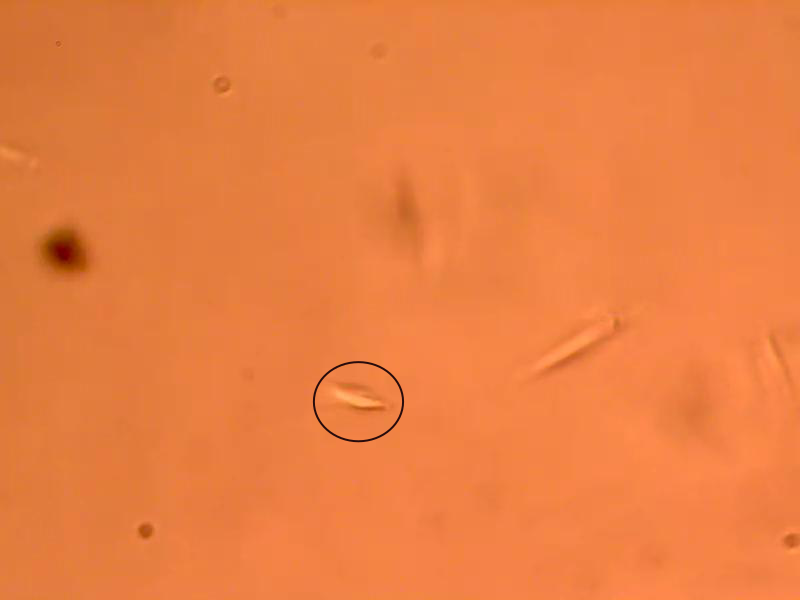
\includegraphics[width=\linewidth ,height=2.3cm]{Results/Resultadosalgea2/firstwatter secondalgea.png} % Renombra tu archivo a este
    \caption*{\textbf{(a)}}
    \label{fig7:a}
    %\vspace{0.1cm}
  \end{subfigure}\hspace{0.5cm} % Espacio horizontal de 0.5cm
  \begin{subfigure}[b]{0.2\linewidth}
    \includegraphics[width=\linewidth ,,height=2.3cm]{Results/Resultadosalgea2/secondalgea2water.png} % Renombra tu archivo a este
    \caption*{\textbf{(b)}}
    \label{fig7:b}
    %\vspace{0.2cm}
  \end{subfigure}

  \begin{subfigure}[b]{0.2\linewidth}
    \includegraphics[width=\linewidth]{Results/Resultadosalgea2/secondalgeawater3.png} % Renombra tu archivo a este
    \caption*{\textbf{(c)}}
    \label{fig7:c}
  \end{subfigure}\hspace{0.5cm} % Espacio horizontal de 0.5cm
  \begin{subfigure}[b]{0.2\linewidth}
    \includegraphics[width=\linewidth]{Results/Resultadosalgea2/secondalgeawater4.png} % Renombra tu archivo a este
    \caption*{\textbf{(d)}}
    \label{fig7:d}
  \end{subfigure}
  \caption{
Manipulación de \textit{Nitzschia Sp.1} (pennada) con el objetivo de inmersión en agua (MO) y un expansor de haz de 10x. La potencia láser se estableció en 25 $mW$. (a-d) Cuadros del video grabado al someter la diatomea al haz láser: (a) Primero, la partícula se encuentra sobre la superficie del portaobjetos con el láser apagado. (b-c) Cuando se enciende el láser, la diatomea comienza a moverse hacia su posición de atrapamiento dentro de las pinzas ópticas (subfigura (d)) debido a la fuerza de gradiente. }
  \label{poresfrustrules}
\end{figure}


}


\only<3>{


\begin{figure}[H]
     \centering
     \begin{subfigure}[b]{0.49\textwidth}
         \centering
         \includegraphics[width=0.6\textwidth]{Results/Resultadosalgea2/oil1.png}
         \caption{}
         \label{fig:y equals x}
     \end{subfigure}
     \hfill
     \begin{subfigure}[b]{0.49\textwidth}
         \centering
         \includegraphics[width=0.60\textwidth]{Results/Resultadosalgea2/oilt2.png}
         \caption{}
         \label{fig:three sin x}
     \end{subfigure}
     \caption{Atrapamiento de \textit{Phaeodactylum tricornutum} (pennada) con el objetivo de inmersión en aceite (MO) y un expansor de haz de 10x. La potencia láser se estableció en 27 $mW$. (a) La diatomea se encuentra sobre la superficie del portaobjetos cuando el láser está apagado. (b) Se enciende el láser y la diatomea alcanza su posición de atrapamiento dentro de las pinzas ópticas debido a la fuerza de gradiente. }
\label{OISECOND2}
     \hfill
    %%
\end{figure}


}

\only<4>{

\begin{figure}
     \centering
     \begin{subfigure}[b]{0.3\textwidth}
         \centering
         \includegraphics[width=\textwidth]{Results/Fifth/pennate1water.png}
         \caption{}
         \label{fig:y equals x}
     \end{subfigure}
     \hfill
     \begin{subfigure}[b]{0.3\textwidth}
         \centering
         \includegraphics[width=\textwidth]{Results/Fifth/pennatewater2.png}
         \caption{}
         \label{fig:three sin x}
     \end{subfigure}
     \hfill
     \begin{subfigure}[b]{0.3\textwidth}
         \centering
         \includegraphics[width=\textwidth]{Results/Fifth/pennate3water.png}
         \caption{}
         \label{fig:five over x}
     \end{subfigure}
       
     \caption{Atrapamiento de \textit{Marine pennate} (pennada) con el objetivo de inmersión en aceite (MO) y un expansor de haz de 2x. La potencia láser se estableció en 232 $mW$. (a-c) Cuadros ordenados cronológicamente del video grabado del atrapamiento de la diatomea pennada mencionada. (a) La diatomea comienza estando sobre la superficie del portaobjetos cuando el láser está apagado. (b-c) Cuando se enciende el láser, la diatomea se mueve hacia su posición de atrapamiento dentro de las pinzas ópticas debido a la fuerza de gradiente.}
\label{WIFORTH1}
     
\end{figure}

}

\only<5>{


\begin{figure}[H]
     \centering
     \begin{subfigure}[b]{0.3\textwidth}
         \centering
         \includegraphics[width=\textwidth]{Results/Resultsforthalgae/falgae1_image2327.png}
         \caption{}
         \label{fig:y equals x}
     \end{subfigure}
     \hfill
     \begin{subfigure}[b]{0.3\textwidth}
         \centering
         \includegraphics[width=\textwidth]{Results/Resultsforthalgae/falgae2.png}
         \caption{}
         \label{fig:three sin x}
     \end{subfigure}
     \hfill
     \begin{subfigure}[b]{0.3\textwidth}
         \centering
         \includegraphics[width=\textwidth]{Results/Resultsforthalgae/falgae3.png}
         \caption{}
         \label{fig:five over x}
     \end{subfigure}
       
     \caption{Atrapamiento de \textit{Navicula Sp.12} con el objetivo de inmersión en agua (MO) (pennada) y un expansor de haz de 10x. La potencia láser se estableció en 31 $mW$. (a-c) Cuadros ordenados cronológicamente del video grabado del atrapamiento de la diatomea \textit{Navicula Sp.12}. (a) La diatomea comienza estando sobre la superficie del portaobjetos cuando el láser está apagado. (b-c) Cuando se enciende el láser, la diatomea se mueve hacia su posición de atrapamiento dentro de las pinzas ópticas debido a la fuerza de gradiente.}
\label{WITHIRD1}
     
\end{figure}




}




\end{frame}

\begin{frame}<1-2>
\frametitle{Resultados}\framesubtitle{Atrapamiento de  diatomea centrica}

\only<1>{


\begin{figure}
  \centering
  \begin{subfigure}[b]{0.2\linewidth}
    \includegraphics[width=\linewidth ,height=2.3cm]{Results/Pseudonana water/wpseudona1.png} % Renombra tu archivo a este
    \caption*{\textbf{(a)}}
    \label{fig7:a}
    %\vspace{0.1cm}
  \end{subfigure}\hspace{0.5cm} % Espacio horizontal de 0.5cm
  \begin{subfigure}[b]{0.2\linewidth}
    \includegraphics[width=\linewidth ,,height=2.3cm]{Results/Pseudonana water/wpseudonana2.png} % Renombra tu archivo a este
    \caption*{\textbf{(b)}}
    \label{fig7:b}
    %\vspace{0.2cm}
  \end{subfigure}

  \begin{subfigure}[b]{0.2\linewidth}
    \includegraphics[width=\linewidth]{Results/Pseudonana water/wpseudonana3.png} % Renombra tu archivo a este
    \caption*{\textbf{(c)}}
    \label{fig7:c}
  \end{subfigure}\hspace{0.5cm} % Espacio horizontal de 0.5cm
  \begin{subfigure}[b]{0.2\linewidth}
    \includegraphics[width=\linewidth]{Results/Pseudonana water/wpseudonana4.png} % Renombra tu archivo a este
    \caption*{\textbf{(d)}}
    \label{fig7:d}
  \end{subfigure}
  \caption{
Atrapamiento de \textit{Thalassiosira pseudonana} (céntrica) con el objetivo de inmersión en agua (MO) y un expansor de haz de 10x. La potencia láser se estableció en 11 $mW$. (a-d) Cuadros del video grabado al someter la diatomea al haz láser: La partícula atrapada permanece inmóvil debido a la acción de la fuerza de gradiente, mientras que las partículas circundantes cambiaron su posición relativa. }
  \label{poresfrustrules}
\end{figure}

}


\only<2>{
\begin{figure}
  \centering
  \begin{subfigure}[b]{0.2\linewidth}
    \includegraphics[width=\linewidth ,height=2.3cm]{Results/ResultsOilpseudonana/op1.png} % Renombra tu archivo a este
    \caption*{\textbf{(a)}}
    \label{fig7:a}
    %\vspace{0.1cm}
  \end{subfigure}\hspace{0.5cm} % Espacio horizontal de 0.5cm
  \begin{subfigure}[b]{0.2\linewidth}
    \includegraphics[width=\linewidth ,,height=2.3cm]{Results/ResultsOilpseudonana/op2.png} % Renombra tu archivo a este
    \caption*{\textbf{(b)}}
    \label{fig7:b}
    %\vspace{0.2cm}
  \end{subfigure}

  \begin{subfigure}[b]{0.2\linewidth}
    \includegraphics[width=\linewidth]{Results/ResultsOilpseudonana/op3.png} % Renombra tu archivo a este
    \caption*{\textbf{(c)}}
    \label{fig7:c}
  \end{subfigure}\hspace{0.5cm} % Espacio horizontal de 0.5cm
  \begin{subfigure}[b]{0.2\linewidth}
    \includegraphics[width=\linewidth]{Results/ResultsOilpseudonana/op4.png} % Renombra tu archivo a este
    \caption*{\textbf{(d)}}
    \label{fig7:d}
  \end{subfigure}
  \caption{
Atrapamiento de \textit{Thalassiosira pseudonana} (céntrica) con el objetivo de inmersión en aceite (MO) y un expansor de haz de 10x. La potencia láser se estableció en 91 $mW$. (a-d) Cuadros del video grabado al someter la diatomea al haz láser: La diatomea atrapada permanece inmóvil debido a la acción de la fuerza de gradiente, mientras que las circundantes cambiaron su posición relativa. }
  \label{poresfrustrules}
\end{figure}

}

\end{frame}


\begin{frame}<1-2>
\frametitle{Results}\framesubtitle{Atrapamiento en microfluidicos}

\only<1>{

\begin{figure}[H]
     \centering
     \begin{subfigure}[b]{0.49\textwidth}
         \centering
         \includegraphics[width=0.95\textwidth]{Newplots_microfluidics_results/Silica_particles.png}
         %surpass the gradient force.
         \caption{Optical tweezers performance for the spherical 6.59 $\mu m$ $SiO_2$ particles.}
         \label{fig:y equals x}
     \end{subfigure}
     \hfill
     \begin{subfigure}[b]{0.49\textwidth}
         \centering
         \includegraphics[width=0.95\textwidth]{Newplots_microfluidics_results/Thala.png}
         \caption{Optical tweezers performance for the \textit{Thalassiosira pseudonana} diatom.}
         \label{fig:three sin x}
     \end{subfigure}
     \caption{Velocidad de flujo umbral promedio (ATFV) para superar la fuerza de gradiente de las pinzas ópticas para (a) partículas esféricas artificiales de sílice y (b) la diatomea \textit{Thalassiosira pseudonana}. El eje vertical representa la velocidad de flujo umbral promedio con desviación estándar $(\sigma)$ para las diferentes potencias láser en el eje horizontal.}
     \hfill
    \label{graficasmicrofluidics} 
\end{figure}


}

\only<2>{\framesubtitle{Calculo de fuerza gradiente}


\begin{figure}[H]
     \centering
     \begin{subfigure}[b]{0.49\textwidth}
         \centering         \includegraphics[width=0.95\textwidth]{Newplots_microfluidics_results/Force_silica_particle.png}
         %surpass the gradient force.
         \caption{Optical tweezers performance for the spherical 6.59 $\mu m$ $SiO_2$ particles.}
         \label{fig:yx}
     \end{subfigure}
     \hfill
     \begin{subfigure}[b]{0.49\textwidth}
         \centering
         \includegraphics[width=0.95\textwidth]{Newplots_microfluidics_results/Force_Thalassiosira.png}
         \caption{Optical tweezers performance for the \textit{Thalassiosira pseudonana} diatom.}
         \label{figx}
     \end{subfigure}
     \caption{Fuerza de arrastre necesaria para superar la fuerza de gradiente de las pinzas ópticas para (a) partículas esféricas artificiales de sílice y (b) la diatomea \textit{Thalassiosira pseudonana}. El eje vertical representa la fuerza de Stokes para las diferentes potencias láser en el eje horizontal.}
     \hfill
    \label{forces_microfluidcs} 
\end{figure}



}


\end{frame}

%trial 


%funciona, pero abre un video extra en un reproductor. 

%\begin{frame}{Video on the computer}
 %   \centering
  %  \movie[externalviewer]{\includegraphics[width=\textheight, keepaspectratio]{logofac.png}}{/home/raymundo/Downloads/circlejonas.mp4}
%\end{frame}




%\begin{frame}{Resultados 1}{Manipulacion de particulas de silica sinteticas}
%-------------------------------------------------------
%\begin{figure}
 %   \centering
  %  \includemovie[autoplay]{12cm}{7cm}{circlejonas.mp4}
   % \caption{2D manipulation of 20.49 $\mu m $ silica particle.}
    %\label{fig:enter-label}
%\end{figure}
  %\begin{itemize}
   % \item Se ha definido el color \textcolor{unamblue}{unamblue}
    %\item Se ha definido el color \textcolor{unamgold}{unamgold}
  %\end{itemize}

%\blfootnote{Se puede usar blfootnote para referencias sin número.}

%\end{frame}

%\begin{frame}{Resultados 1}{Atrapamiento de celulas de levadura.}
%-------------------------------------------------------

%\begin{block}{Bloque de texto}
 % \begin{itemize}
  %  \item Información 1
   % \item Información 2
    %\item Información 3
    %\item Información 4
  %\end{itemize}
%\end{block}

%\blfootnote{Autor, D. Int. J. Quantum Power, 152(1), 125-130 (2023)}

%\end{frame}
\begin{comment}
%\begin{frame}{Resultados 1}{Ejecucion por luz de las celulas de levaudra.}
%Ejemplifica el efecto detrimental de la radiacion en las celulas vivas.
%\end{frame}





%\begin{frame}{Resultados 2}{Cuantificacion de fuerzas}
    
%\end{frame}

\end{comment}
%-------------------------------------------------------
\section{Conclusiones}
%-------------------------------------------------------
\begin{frame}<1-4>\frametitle{Conclusiones}
%-------------------------------------------------------
\only<1>{
\begin{itemize}
    \item \textbf{Primera parte – Manipulación de partículas artificiales:}
    \begin{itemize}
        \item Se usaron partículas de sílice esféricas (4.25 µm y 4.27 µm) para manipulación 3D.
        \item Partículas más grandes (19.98 µm y 24.82 µm) solo pudieron manipularse en 2D.
      %  \item Manipulación 3D de células de levadura, formando patrones sobre el portaobjetos.
       % \item Se observó muerte celular inducida por luz (\textit{opticution}) a diferentes potencias láser.
    \end{itemize}
\end{itemize}



}


\only<2>{



\begin{itemize}    
    \item \textbf{Segunda parte – Aplicación a organismos biológicos:}
    \begin{itemize}
            \item Manipulación 3D de células de levadura, formando patrones sobre el portaobjetos.
        \item Se observó muerte celular inducida por luz (\textit{opticution}).
        \item Manipulación de especies de diatomeas: \textit{Nitzchia sp.1}, \textit{Phaeodactylum tricornutum}, \textit{Navicula Sp.12}, \textit{Marine pennate} y \textit{Thalassiosira pseudonana}.
        %\item Diatomeas con simetría bilateral tendieron a rotar y alinear su eje con el eje vertical.
    \end{itemize}
    
    \item \textbf{Uso de dispositivos microfluídicos:}
    \begin{itemize}
        \item Medición de la velocidad del fluido necesaria para liberar partículas atrapadas.
        \item Cálculo de la fuerza de gradiente a partir de la fuerza de Stokes.
        %\item Fuerzas experimentales mayores que las teóricas, posibles causas:

    \end{itemize}
\end{itemize}





}


\only<3>{

\begin{figure}[H]
    \centering
    \includegraphics[width=0.5\textwidth]{profile.png}
    \caption{Perfil de velocidad de un fluido}
    \label{fig:etiqueta}
\end{figure}

}

\only<4>{
\begin{itemize}

    \item \textbf{Perspectivas futuras:}
    \begin{itemize}
        \item Estudios detallados de células individuales de diatomeas.
        %\item Modelado más preciso usando teoría de Lorenz-Mie generalizada.
        \item Comparaciones con distintas longitudes de onda y aumentos.
        \item Estudio de reproducción al cambiar el medio durante el atrapamiento.
      %  \item Uso de infrarrojo para evitar fotodaño por radiación.
        \item Estudios espectroscópicos del frústulo para analizar su protección frente a luz UV.
    \end{itemize}
    \end{itemize}

}

\end{frame}
%\section*{Extra slides}
%\begin{frame}{Presion radiacion}{Subtítulo Genérico}
%-------------------------------------------------------

%  \begin{itemize}
 %   \item Se ha definido el color \textcolor{unamblue}{unamblue}
  %  \item Se ha definido el color \textcolor{unamgold}{unamgold}
  %\end{itemize}

%\blfootnote{Se puede usar blfootnote para referencias sin número.}

%\end{frame}




\end{document}
